% This file is a template using the "beamer" package to create slides for a talk or presentation
% - Talk at a conference/colloquium.
% - Talk length is about 20min.
% - Style is ornate.


% draft包的作用是在编译时不生成目录、图片、超链接等,只处理文字和排版(未显示内容用同等大小的灰色方框替代)
% 这样可以在编辑文档查看效果时加快编译速度
% 但是在确定文档内容后,需要删除draft包(使用下一行documentclass),否则目录不会生成。
% \documentclass[aspectratio=169, UTF8, draft]{beamer}
\documentclass[aspectratio=169, UTF8]{beamer}

\usepackage{ctex} % 中文支持
\usepackage{multicol} % 多栏支持
\usepackage{graphicx}
\usepackage{caption}
\usepackage{listings} % 代码高亮
\usetheme{Kokura}

\usepackage[english]{babel} % 在toc中显示英文

% 在封面页需要展示的信息
\title{\textbf{Image Segmentation Based on Deep Neural Network and Active Contour Model}}
% \subtitle{一份毕业答辩Beamer演示文稿示例} % 可选
\author{\textbf{Alex Xu}}
%\institute{\textbf{计算机与通信工程学院}}
%\date{2024年6月18日}

% Delete this, if you do not want the table of contents to pop up at
% the beginning of each subsection:
% \AtBeginSubsection[]
% {
  % \begin{frame}<beamer>{Outline}
    % \tableofcontents[currentsection,currentsubsection]
  % \end{frame}
% }

\begin{document}
% 默认在title page中加入图片background.png
{
  \usebackgroundtemplate{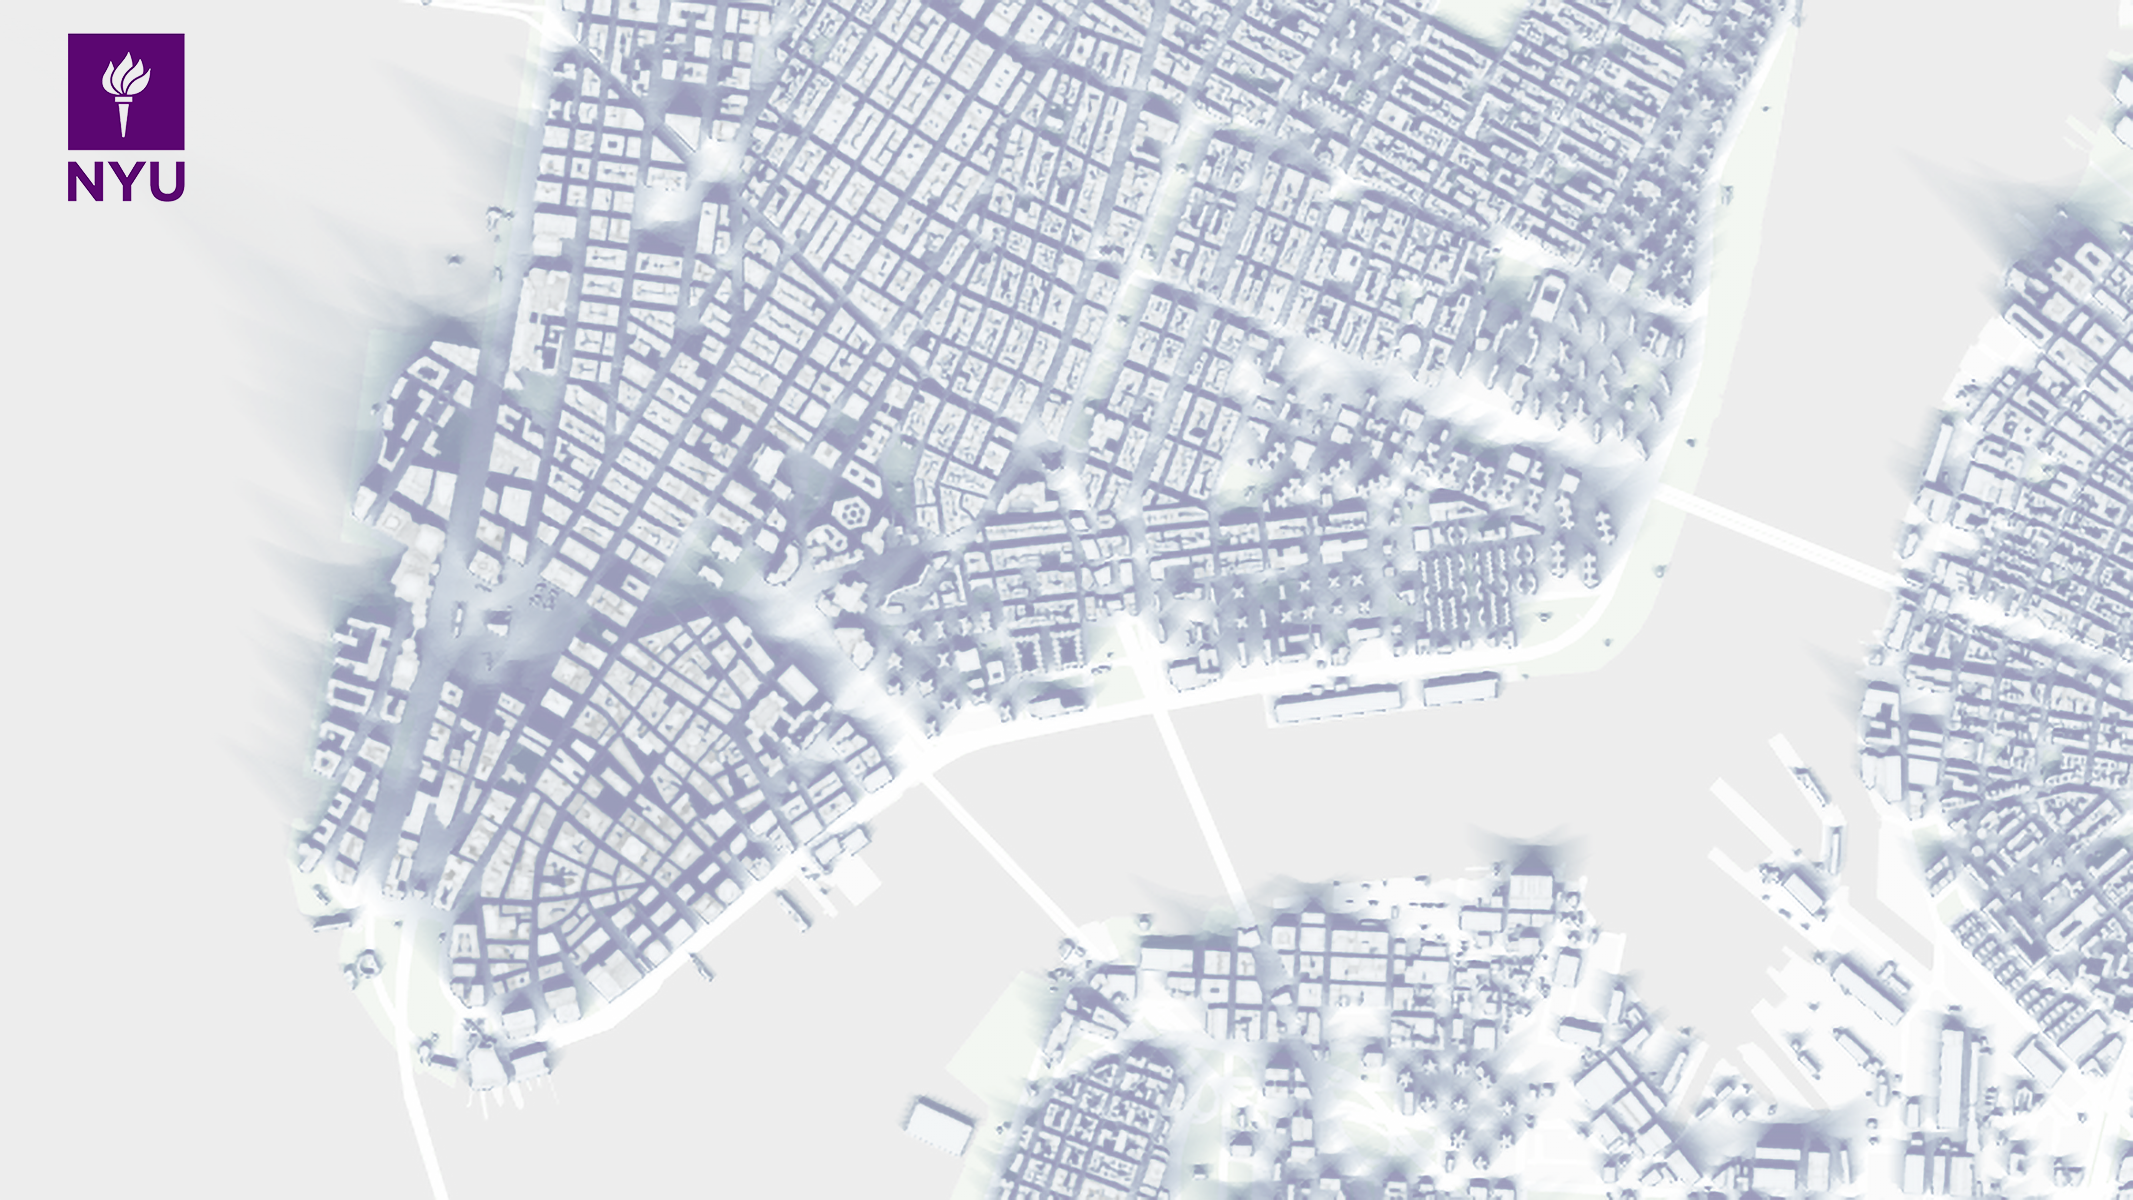
\includegraphics[width=\paperwidth]{background_purple_nyu.png}} % 背景图片
  \begin{frame}[plain, noframenumbering]
    \titlepage
  \end{frame}
}

% 如果不需要背景图片,可以使用下面的命令
% \begin{frame}[plain, noframenumbering]
  % \titlepage
% \end{frame}

% 目录自动生成,显示所有的section和subsection
\begin{frame}[plain, allowframebreaks, noframenumbering]{Content}
  % \begin{multicols}{2} % 多栏显示
  %   \tableofcontents[]%
  % \end{multicols}
  % 如果想要单栏显示目录,可以使用下面的命令
  \tableofcontents
\end{frame}

% 内容主体
\section{Basic theory}

\subsection{Overview}
\begin{frame}{Background}
	\begin{itemize}[<+->]
		\item Overview of image segmentation.
		\item Traditional: Accurate segmentation by Active Contour Model.
		\item Innovation: Deep learning methods.
	\end{itemize}
\end{frame}

\subsection{Mathematical Derivation}
\begin{frame}{Active Contour Model}
	\begin{block}{Curve evolution}
		We define curve as
		\begin{equation}
			\mathrm{C}(\theta,t)=(x(\theta,t),y(\theta,t))
		\end{equation}
		Then we have curvature
		\begin{equation}
			\frac{\partial \mathrm{C}(\theta,t)}{\partial t}=\mathrm{F}(k)N
		\end{equation}
		As constant evolution
		\begin{equation}
			\frac{\partial \mathrm{C}(\theta,t)}{\partial t}=V_0 N
		\end{equation}
		As curvature evolution
		\begin{equation}
			\frac{\partial \mathrm{C}(\theta,t)}{\partial t}=\alpha k N
		\end{equation}
	\end{block}
\end{frame}

\begin{frame}{Active Contour Model}
	\begin{block}{Level-set method}
		In curve $\mathrm{C}=\{(x,y),\phi(x,y)=c\}$ where $\phi(x,y)$ defined as level-set function, we introduce time $t$ and apply partial derivatives
		\begin{equation}
			\frac{\mathrm{d} \phi}{\mathrm{d} t}=\frac{\partial \phi}{\partial t}+\frac{\partial \phi}{\partial x}\cdot\frac{\partial x}{\partial t}+\frac{\partial \phi}{\partial y}\cdot\frac{\partial y}{\partial t}=\frac{\partial \phi}{\partial t}+\nabla\phi\cdot\frac{\partial (x,y)}{\partial t}=0
		\end{equation}
		$\nabla\phi=(\frac{\partial \phi}{\partial x},\frac{\partial \phi}{\partial y})$ is the gradient of level set function $\phi(x,y)$, and $\frac{\partial (x,y)}{\partial t}=\frac{\partial \mathrm{C}}{\partial t}=(\frac{\partial x}{\partial t},\frac{\partial y}{\partial t})=\vec{V}$. Then
		\begin{equation}
			\frac{\partial \phi}{\partial t}=-\nabla \phi \cdot \vec{V}=-|\nabla \phi| \cdot \frac{\vec{V}}{\nabla \phi}=|\nabla \phi| \cdot\left(-\frac{\nabla \phi}{|\nabla \phi|}\right) \cdot \vec{V}=|\nabla \phi| \cdot \vec{U} \cdot \vec{V}
		\end{equation}
	\end{block}
\end{frame}

\begin{frame}{Active Contour Model}
	\begin{block}{Calculus of variations}
		The 1D energy function can be written as
		\begin{equation}
			\mathrm{E}(\phi)=\int_{x_0}^{x_1}\mathrm{F}(x,\phi,\phi^\prime)\mathrm{d}x
		\end{equation}
		In order to apply Taylor's Formula, we introduce a very small $v(x)$
		\begin{equation}
			\mathrm{F}(x,\phi+v,\phi^\prime+v^\prime)=\mathrm{F}(x,\phi,\phi^\prime)+\frac{\partial \mathrm{F}}{\partial \phi}\cdot v+\frac{\partial \mathrm{F}}{\partial \phi^\prime}\cdot v+\cdots
		\end{equation}
		Intergrate both sides and collate to get
		\begin{equation}
			\mathrm{E}(\phi+v)-\mathrm{E}(\phi)=\int_{x_0}^{x_1}\left(v \frac{\partial \mathrm{F}}{\partial \phi}+v^{\prime} \frac{\partial \mathrm{F}}{\partial \phi^{\prime}}\right) \mathrm{d} x
		\end{equation}
	\end{block}
\end{frame}

\begin{frame}{Active Contour Model}
	\begin{block}{Calculus of variations}
		As $\phi(x_0)+v(x_0)=a,\phi(x_1)+v(x_1)=b$,
		\begin{equation}
			\int_{x_0}^{x_1} v^{\prime} \frac{\partial \mathrm{F}}{\partial \phi^{\prime}} \mathrm{d} x=\int_{x_0}^{x_1} \frac{\partial \mathrm{F}}{\partial \phi} \mathrm{d} v=\left.v \frac{\partial \mathrm{F}}{\partial \phi^{\prime}}\right|_{x_0} ^{x_1}-\int_{x_0}^{x_1} v \frac{\mathrm{d}}{\mathrm{d} x} \frac{\partial \mathrm{F}}{\partial \phi^{\prime}} \mathrm{d} x=-\int_{x_0}^{x_1} v \frac{\mathrm{d}}{\mathrm{d} x} \frac{\partial \mathrm{F}}{\partial \phi^{\prime}} \mathrm{d} x
		\end{equation}
		Ignoring very small changes in the independent variable, we have
		\begin{equation}
			\frac{\partial \mathrm{F}}{\partial \phi}-\frac{\mathrm{d}}{\mathrm{d}x}(\frac{\partial \mathrm{F}}{\partial \phi^\prime})=0
			\label{eq:1d}
		\end{equation}
		This is the Euler equation for 1D energy functional. Similarly, The Euler equation for 2D is
		\begin{equation}
			\frac{\partial \mathrm{F}}{\partial \phi}-\frac{\partial \mathrm{F}}{\partial \phi_x}-\frac{\partial \mathrm{F}}{\partial \phi_y}=0
		\end{equation}
	\end{block}
\end{frame}

\begin{frame}{Active Contour Model}
	\begin{block}{Calculus of variations}
		Take (\ref{eq:1d}) as an example. To solve the Euler equation, we introduce a small $v(\cdot)$
		\begin{equation}
			\mathrm{E}(\phi, t+\Delta t)=\mathrm{E}(\phi, t)+\Delta t \int_{x_0}^{x_1} \frac{\partial \phi}{\partial t}\left(\frac{\partial \mathrm{F}}{\partial \phi}-\frac{\mathrm{d}}{\mathrm{d} x}\left(\frac{\partial \mathrm{F}}{\partial \phi^{\prime}}\right)\right) \mathrm{d} x
		\end{equation}
		Let
		\begin{equation}
			\frac{\partial \phi}{\partial t}=-\left(\frac{\partial \mathrm{F}}{\partial \phi}-\frac{\mathrm{d}}{\mathrm{d} x}\left(\frac{\partial \mathrm{F}}{\partial \phi^{\prime}}\right)\right)=\frac{\mathrm{d}}{\mathrm{d} x}\left(\frac{\partial \mathrm{F}}{\partial \phi^{\prime}}\right)-\frac{\partial \mathrm{F}}{\partial \phi}
		\end{equation}
		Then
		\begin{equation}
			\Delta \mathrm{E}=\mathrm{E}(\phi,t+\Delta t)-\mathrm{E}(\phi,t)=-\Delta t\int\left(\frac{\partial \mathrm{F}}{\partial \phi}-\frac{\mathrm{d}}{\mathrm{d} x}\left(\frac{\partial \mathrm{F}}{\partial \phi^{\prime}}\right)\right)^2\mathrm{d}x
		\end{equation}
		The solution to the Euler equation of an energy functional tends to stabilize as the curve evolves, corresponding to the gradient flow of the given variation.
	\end{block}
\end{frame}

\begin{frame}{Active Contour Model}
	\begin{block}{Chan Vese Model}
		Chan and Vese proposed the Chan-Vese active contour model. Given a grayscale image $I(x)$, the target $\Omega_1$ and background $\Omega_2$ are detected with characteristic uniformity and a clear difference, represented by the approximate grayscale constants $c_1$ and $c_2$. The energy functional is defined as
		\begin{equation}
			\begin{aligned}
				\mathrm{F}\left(c_1, c_2, \phi\right) & =\lambda_1 \cdot \int_{\Omega}\left(\mathrm{I}(x)-c_1\right)^2 \cdot \mathrm{H}(\phi(x)) \mathrm{d} x+\lambda_2 \cdot \int_{\Omega}\left(\mathrm{I}(x)-c_2\right)^2 \cdot(1-\mathrm{H}(\phi(x))) \mathrm{d} x \\
				& +\mu \cdot \int_{\Omega} \delta_0(\phi(x))|\nabla \phi(x)| \mathrm{d} x+v \cdot \int_{\Omega} \mathrm{H}(\phi(x)) \mathrm{d} x
			\end{aligned}
		\end{equation}
		Where $\lambda_1,\lambda_2>0,\mu,v\geq0$. $\mathrm{H}(\phi)$ is the unit step function(Heaviside function). $\delta_0$ is its derivative, from which the Dirac function can be derived.
		\begin{equation}
			\mathrm{H}(z)=\left\{\begin{array}{ll}
				0 & z<0 \\
				1 & z \geq 0
			\end{array}, \delta_0(z)=\frac{\mathrm{d}}{\mathrm{d} z} \mathrm{H}(z)\right.
		\end{equation}
	\end{block}
\end{frame}

\begin{frame}{Active Contour Model}
	\begin{block}{Chan Vese Model}
		Substituting it into the Euler-Lagrange equation, the level set gradient flow of the Chan-Vese model is solved.
		\begin{equation}
			\frac{\partial \phi}{\partial \mathrm{t}}=-\frac{\partial \mathrm{F}}{\partial \phi}=\delta_{\varepsilon}\left\lfloor\mu \operatorname{div}\left(\frac{\nabla \phi}{|\nabla \phi|}\right)-v-\lambda_1\left(\mathrm{I}(x)-c_1\right)^2+\lambda_2\left(\mathrm{I}(x)-c_2\right)^2\right\rfloor
		\end{equation}
		where
		\begin{equation}
			c_1=\frac{\int \mathrm{I}(x) \cdot H(\phi(x)) \mathrm{d} x}{\int \mathrm{H}(\phi(x)) \mathrm{d} x}, \quad c_2=\frac{\int \mathrm{I}(x) \cdot(1-\mathrm{H}(\phi(x))) \mathrm{d} x}{\int(1-\mathrm{H}(\phi(x))) \mathrm{d} x}
		\end{equation}
	\end{block}
\end{frame}

\subsection{Dive into Deep Learning}
\begin{frame}{Neural Network}
	\begin{block}{Convolutional Neural Networks}
		\begin{itemize}
			\item convolutional layer
			\item pooling layer
			\item flatten layer
			\item fully connected layer
			\item activation layer
		\end{itemize}
	\end{block}
\end{frame}

\begin{frame}{Neural Network}
	\begin{figure}[h]
		\centering
		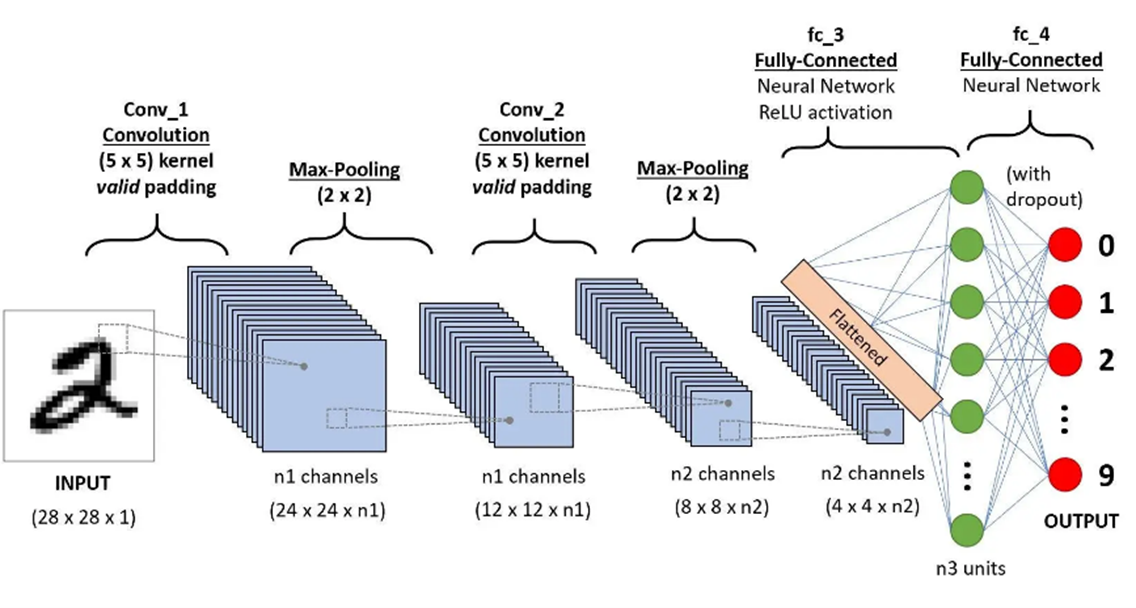
\includegraphics[width=0.8\textwidth]{images/num_rec.png}
		\caption{Handwritten number recognition pipeline}
		\label{fig:num_rec}
	\end{figure}
\end{frame}

\begin{frame}{Loss Functions}
	\begin{columns}
		\begin{column}{0.25\textwidth}
			\begin{block}{Softmax}
				\begin{equation}
					\text{Softmax}(x)=\frac{e^{x_i}}{\sum_i e^{x_i}}
				\end{equation}
			\end{block}
		\end{column}
		\pause
		\begin{column}{0.25\textwidth}
			\begin{block}{Sigmoid}
				\begin{equation}
					\text{Sigmoid}(x)=\frac{1}{1+e^{-x}}
				\end{equation}
			\end{block}
		\end{column}
		\pause
		\begin{column}{0.25\textwidth}
			\begin{block}{tanh}
				\begin{equation}
					\text{tanh}(x)=\frac{e^x-e^{-x}}{e^x+e^{-x}}
				\end{equation}
			\end{block}
		\end{column}
		\pause
		\begin{column}{0.25\textwidth}
			\begin{block}{ReLU}
				\begin{equation}
					\text{ReLU}(x)=\max(0,x)
				\end{equation}
			\end{block}
		\end{column}
	\end{columns}
\end{frame}

\begin{frame}{Optimizations}
	\begin{block}{Methods}
		\begin{itemize}
			\item Batch normalization
			\begin{equation}
				{\hat{x}}_i=\frac{x_i-\mu_B}{\sqrt{\sigma^2_B+\varepsilon}}
			\end{equation}
			\item Stochastic gradient descent
			\begin{equation}
				\theta=\theta-\eta\cdot\nabla_\theta J(\theta,x^{(i)},y^{(i)})
			\end{equation}
		\end{itemize}
	\end{block}
\end{frame}

\begin{frame}{Classic Models}
	\begin{columns}
		\begin{column}{0.5\textwidth}
			\begin{figure}[h]
				\centering
				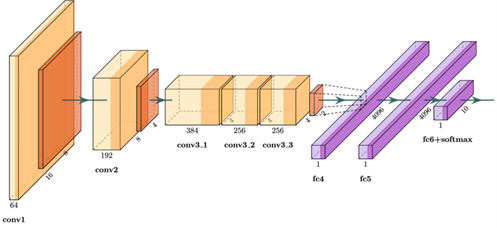
\includegraphics[width=0.75\columnwidth]{images/alexnet.png}
				\caption{AlexNet}
				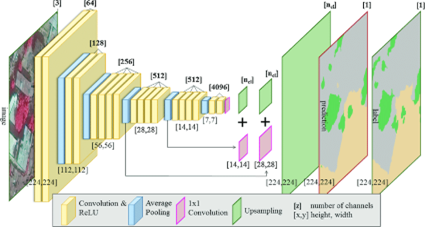
\includegraphics[width=0.7\columnwidth]{images/fcn.png}
				\caption{FCN}
			\end{figure}
		\end{column}
		\begin{column}{0.5\textwidth}
			\begin{figure}[h]
				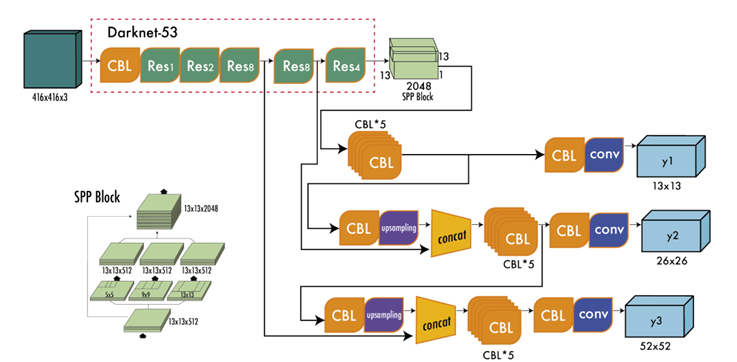
\includegraphics[width=0.7\columnwidth]{images/darknet.png}
				\caption{DarkNet}
				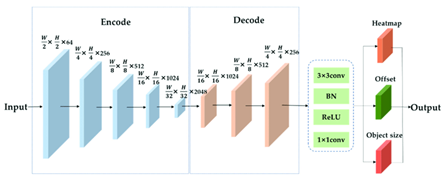
\includegraphics[width=0.75\columnwidth]{images/centernet.png}
				\caption{CenterNet}
			\end{figure}
		\end{column}
	\end{columns}
\end{frame}







\begin{frame}[plain, allowframebreaks, noframenumbering]{Content}
	\tableofcontents
\end{frame}

\section{Methodology}

%\subsection{分栏显示}
\subsection{From R-CNN to YOLO}
\begin{frame}{R-CNN Series}
    \begin{columns}
        \begin{column}{0.5\textwidth}
            R-CNN is an object detection model that uses selective search for region proposals, feeds these into a pre-trained CNN for feature extraction, and then classifies and refines the regions using SVMs and bounding box regressors. \\
            \bigskip
            It laid the foundation for deep learning-based object detection but was computationally intensive.

        \end{column}
        \begin{column}{0.5\textwidth}
            \begin{figure}[h]
                \centering
                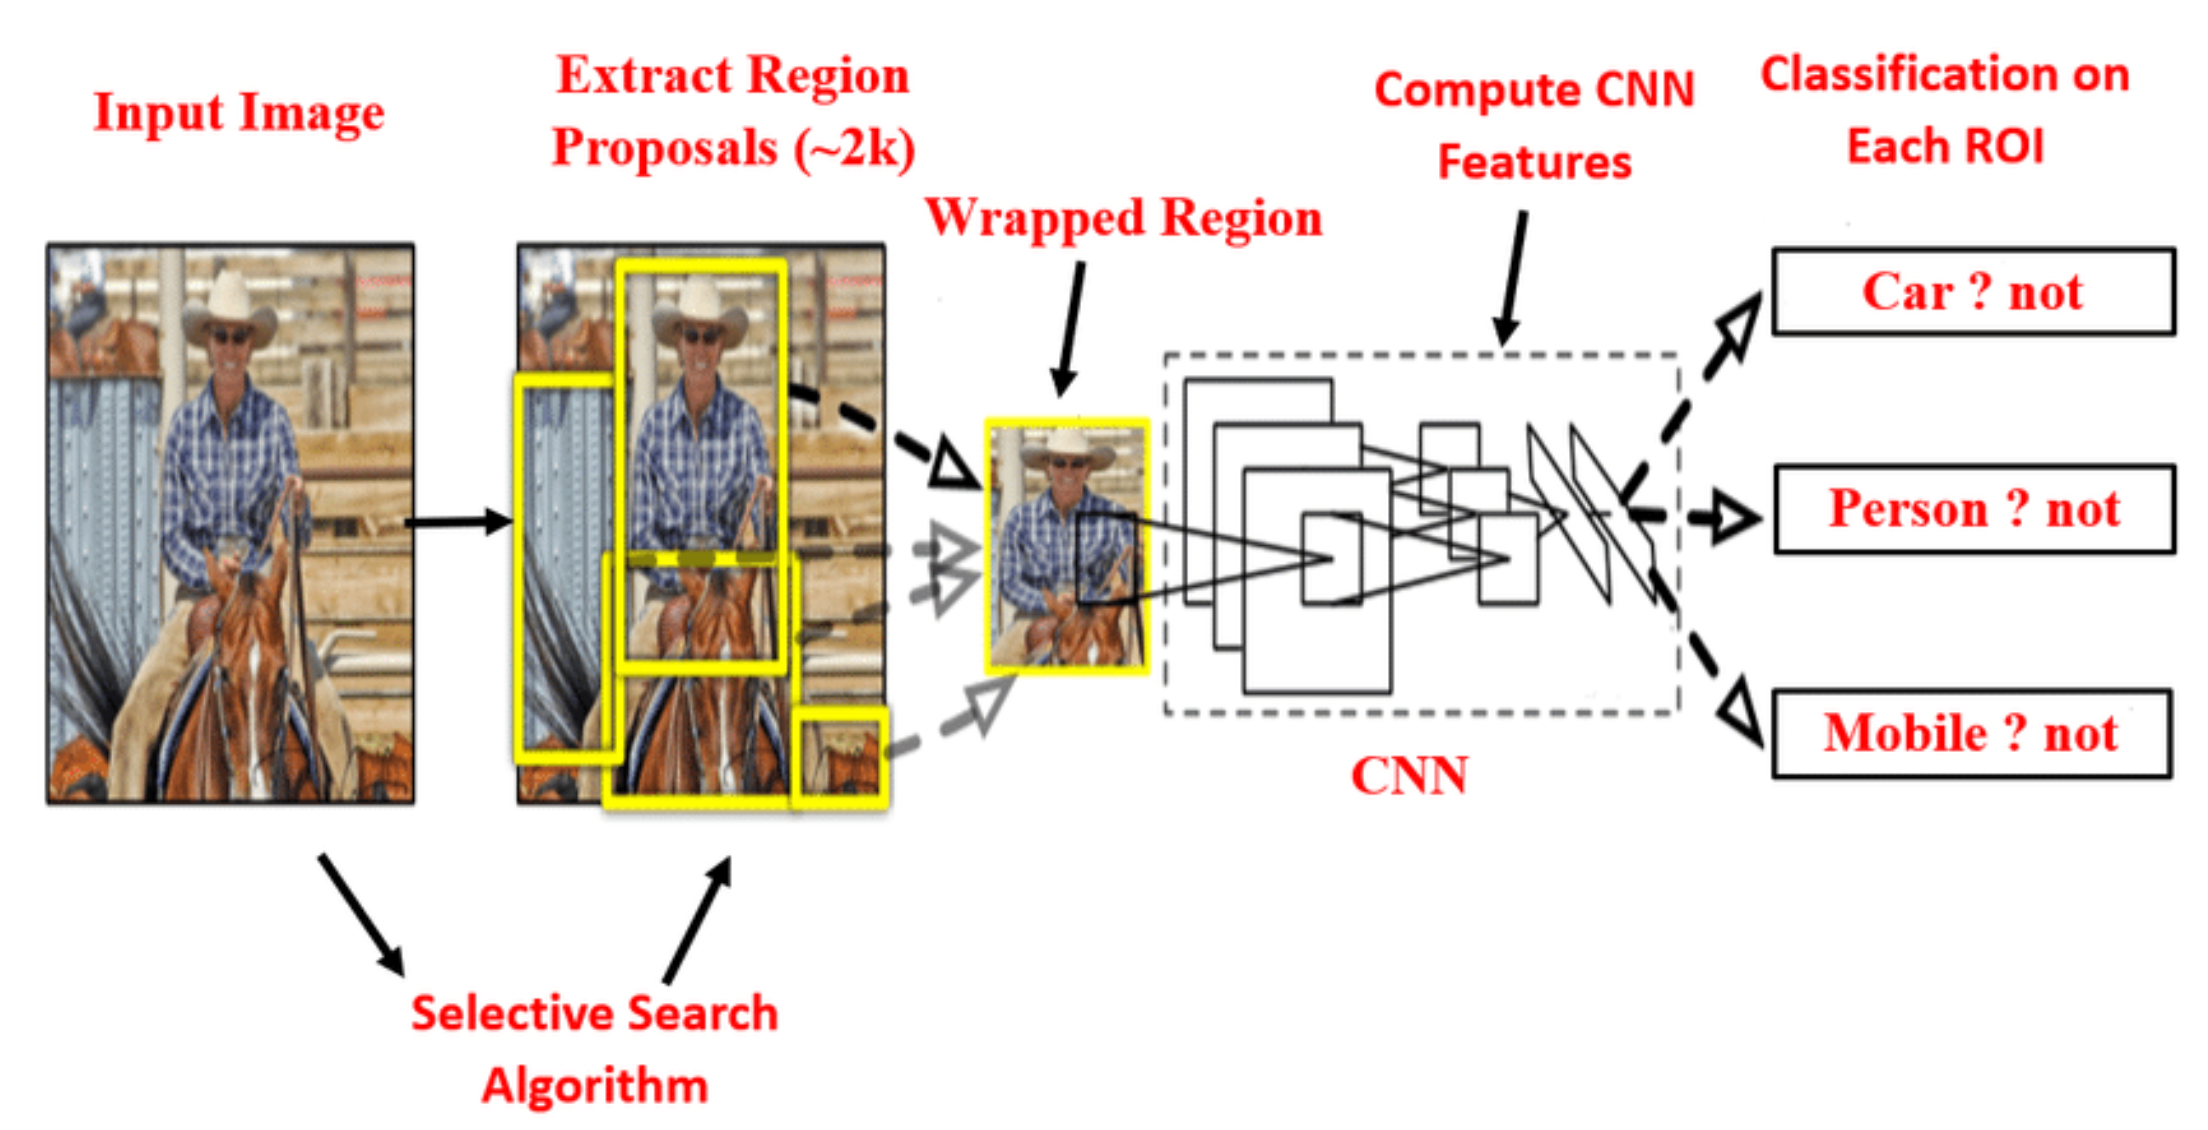
\includegraphics[width=\textwidth]{images/rcnn.png}
                \caption{R-CNN}
                \label{fig:rcnn}
            \end{figure}
        \end{column}
    \end{columns}
\end{frame}

\begin{frame}{R-CNN series}
	\begin{columns}
		\begin{column}{0.5\textwidth}
			\begin{figure}[h]
				\centering
				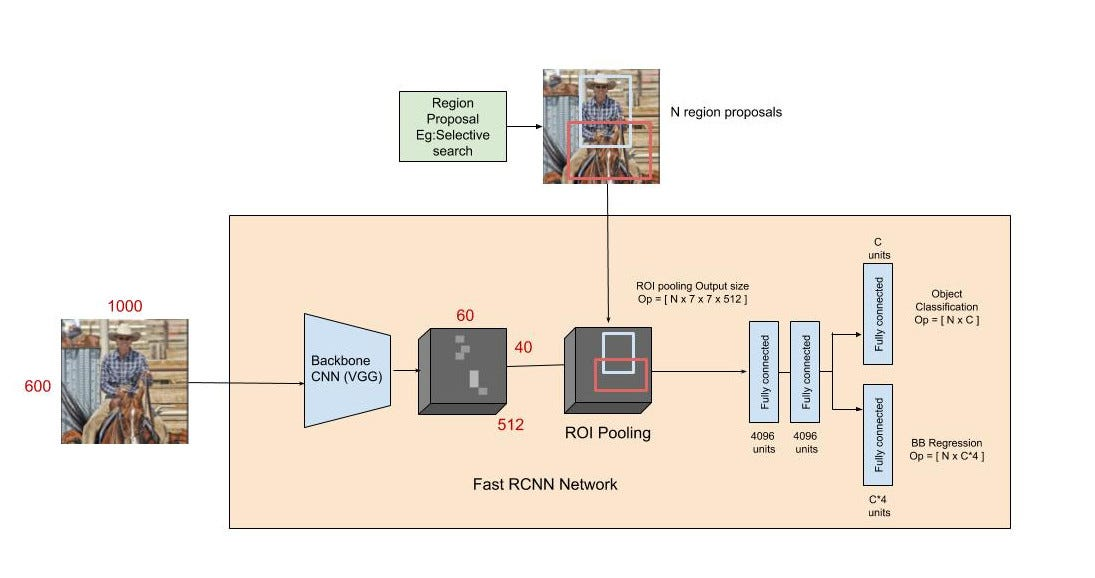
\includegraphics[width=\textwidth]{images/fast-rcnn.jpeg}
				\caption{Fast R-CNN}
				\label{fig:fast-rcnn}
			\end{figure}
		\end{column}
		\begin{column}{0.5\textwidth}
			\begin{figure}[h]
				\centering
				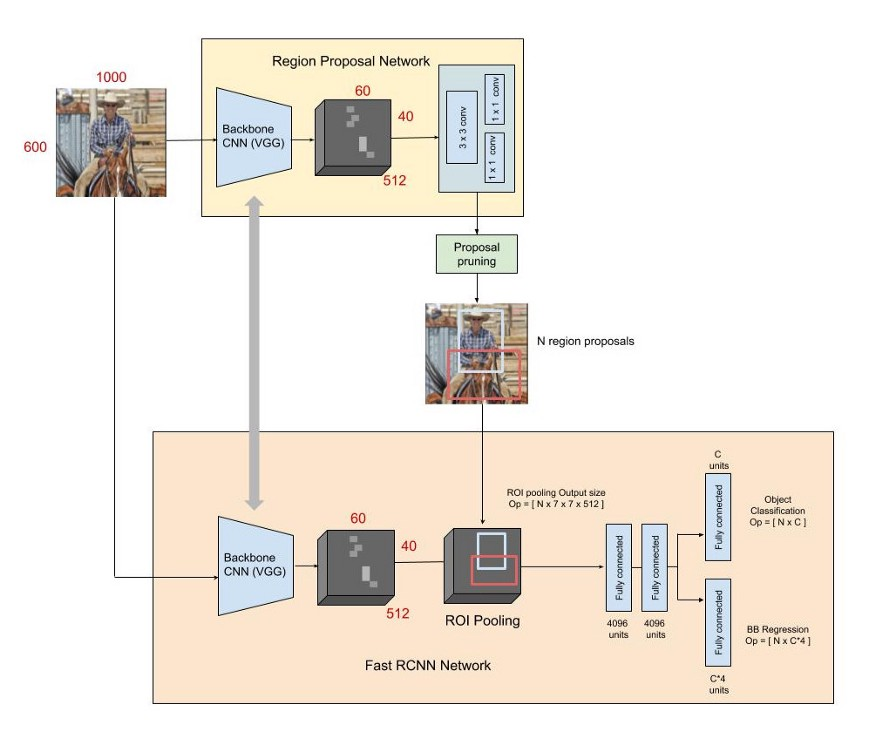
\includegraphics[width=\textwidth]{images/faster-rcnn.jpeg}
				\caption{Faster R-CNN}
				\label{fig:faster-rcnn}
			\end{figure}
		\end{column}
	\end{columns}
\end{frame}

\begin{frame}{You Only Look Once}
	\begin{columns}
		\begin{column}{0.43\textwidth}
			\begin{block}{Innovations}
				\begin{itemize}
				\item Unified detection framework
				\item Real-time detection
				\item Global contextual prediction
				\item Spatially separated bounding boxes
				\item End-to-end training
			\end{itemize}
			\end{block}
		\end{column}
		\begin{column}{0.57\textwidth}
			\begin{figure}[h]
				\centering
				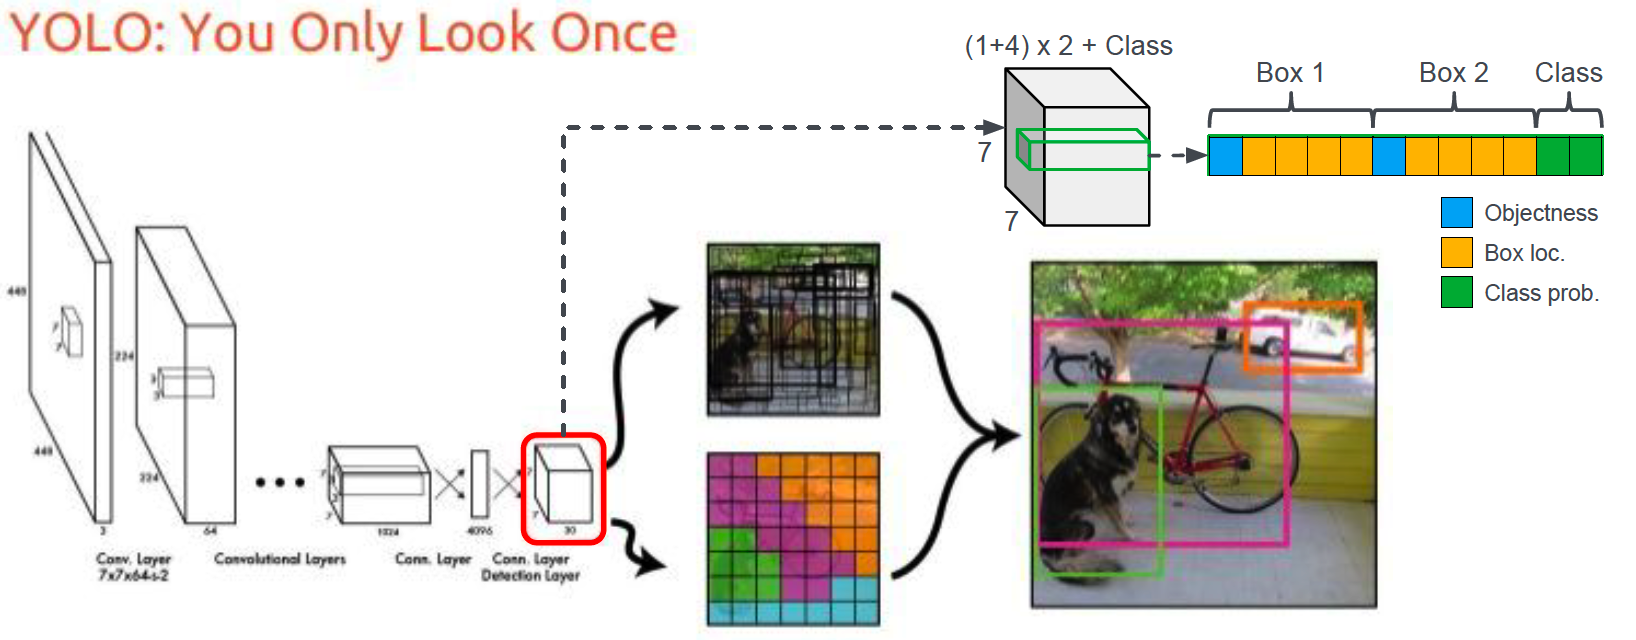
\includegraphics[width=\textwidth]{images/yolov1.png}
				\caption{YOLOv1 architecture}
				\label{fig:yolov1}
			\end{figure}
		\end{column}
	\end{columns}
\end{frame}

\begin{frame}{Loss Function Improvement}
	\begin{block}{YOLOv1}
		\begin{equation}
			\begin{aligned}
				\text { Loss }= & \lambda_{\text {coord }} \sum_{i=0}^{S^2} \sum_{j=0}^B I_{i j}^{\mathrm{obj}}\left[\left(x_i^j-\hat{x}_i^j\right)^2+\left(y_i^j-\hat{y}_i^j\right)^2\right] \\
				& +\lambda_{\text {coord }} \sum_{i=0}^{S^2} \sum_{j=0}^B I_{i j}^{\text {obj }}\left[\left(\sqrt{w_i^j}-\sqrt{\hat{w}_i^j}\right)^2+\left(\sqrt{h_i^j}-\sqrt{\hat{h}_i^j}\right)^2\right] \\
				& +\sum_{i=0}^{s^2} \sum_{j=0}^B I_{i j}^{\text {obj }}\left(C_i^j-\hat{C}_i^j\right)^2 \\
				& +\lambda_{\text {noobj }} \sum_{i=0}^{S^2} \sum_{j=0}^B I_{i j}^{\text {noobj }}\left(C_i^j-\hat{C}_i^j\right)^2 \\
				& +\sum_{i=0}^{s^2} I_{i j}^{\text {obj }} \sum_{c \in \text { classes }}\left(P_i^j(c)-\hat{C}_i^j(c)\right)^2
			\end{aligned}
		\end{equation}
	\end{block}
\end{frame}

\begin{frame}{Loss Function Improvement}
	\begin{block}{YOLOv3}
		\begin{equation}
			\begin{aligned}
				\text { Loss }= & \lambda_{\text {coord }} \sum_{i=0}^{S^2} \sum_{j=0}^B I_{i j}^{\mathrm{obj}}\left[\left(x_i^j-\hat{x}_i^j\right)^2+\left(y_i^j-\hat{y}_i^j\right)^2\right] \\
				& +\lambda_{\text {coord }} \sum_{i=0}^{S^2} \sum_{j=0}^B I_{i j}^{\mathrm{obj}}\left[\left(\sqrt{w_i^j}-\sqrt{\hat{w}_i^j}\right)^2+\left(\sqrt{h_i^j}-\sqrt{\hat{h}_i^j}\right)^2\right] \\
				& -\sum_{i=0}^{s^2} \sum_{j=0}^B I_{i j}^{\mathrm{obj}}\left[\hat{C}_i^j \log \left(C_i^j\right)+\left(1-\hat{C}_i^j\right) \log \left(1-C_i^j\right)\right] \\
				& -\lambda_{\text {noobj }} \sum_{i=0}^{S^2} \sum_{j=0}^B I_{i j}^{\mathrm{noobj}}\left[\hat{C}_i^j \log \left(C_i^j\right)+\left(1-\hat{C}_i^j\right) \log \left(1-C_i^j\right)\right] \\
				& -\sum_{i=0}^{s^2} I_{i j}^{\mathrm{obj}} \sum_{c \in \text { classes }}\left[\hat{P}_i^j \log \left(P_i^j\right)+\left(1-\hat{P}_i^j\right) \log \left(1-P_i^j\right)\right]
			\end{aligned}
		\end{equation}
	\end{block}
\end{frame}

\subsection{The Greatest Works}
\begin{frame}{Masterpieces}
	\begin{columns}
		\begin{column}{0.5\textwidth}
			\begin{figure}[h]
				\centering
				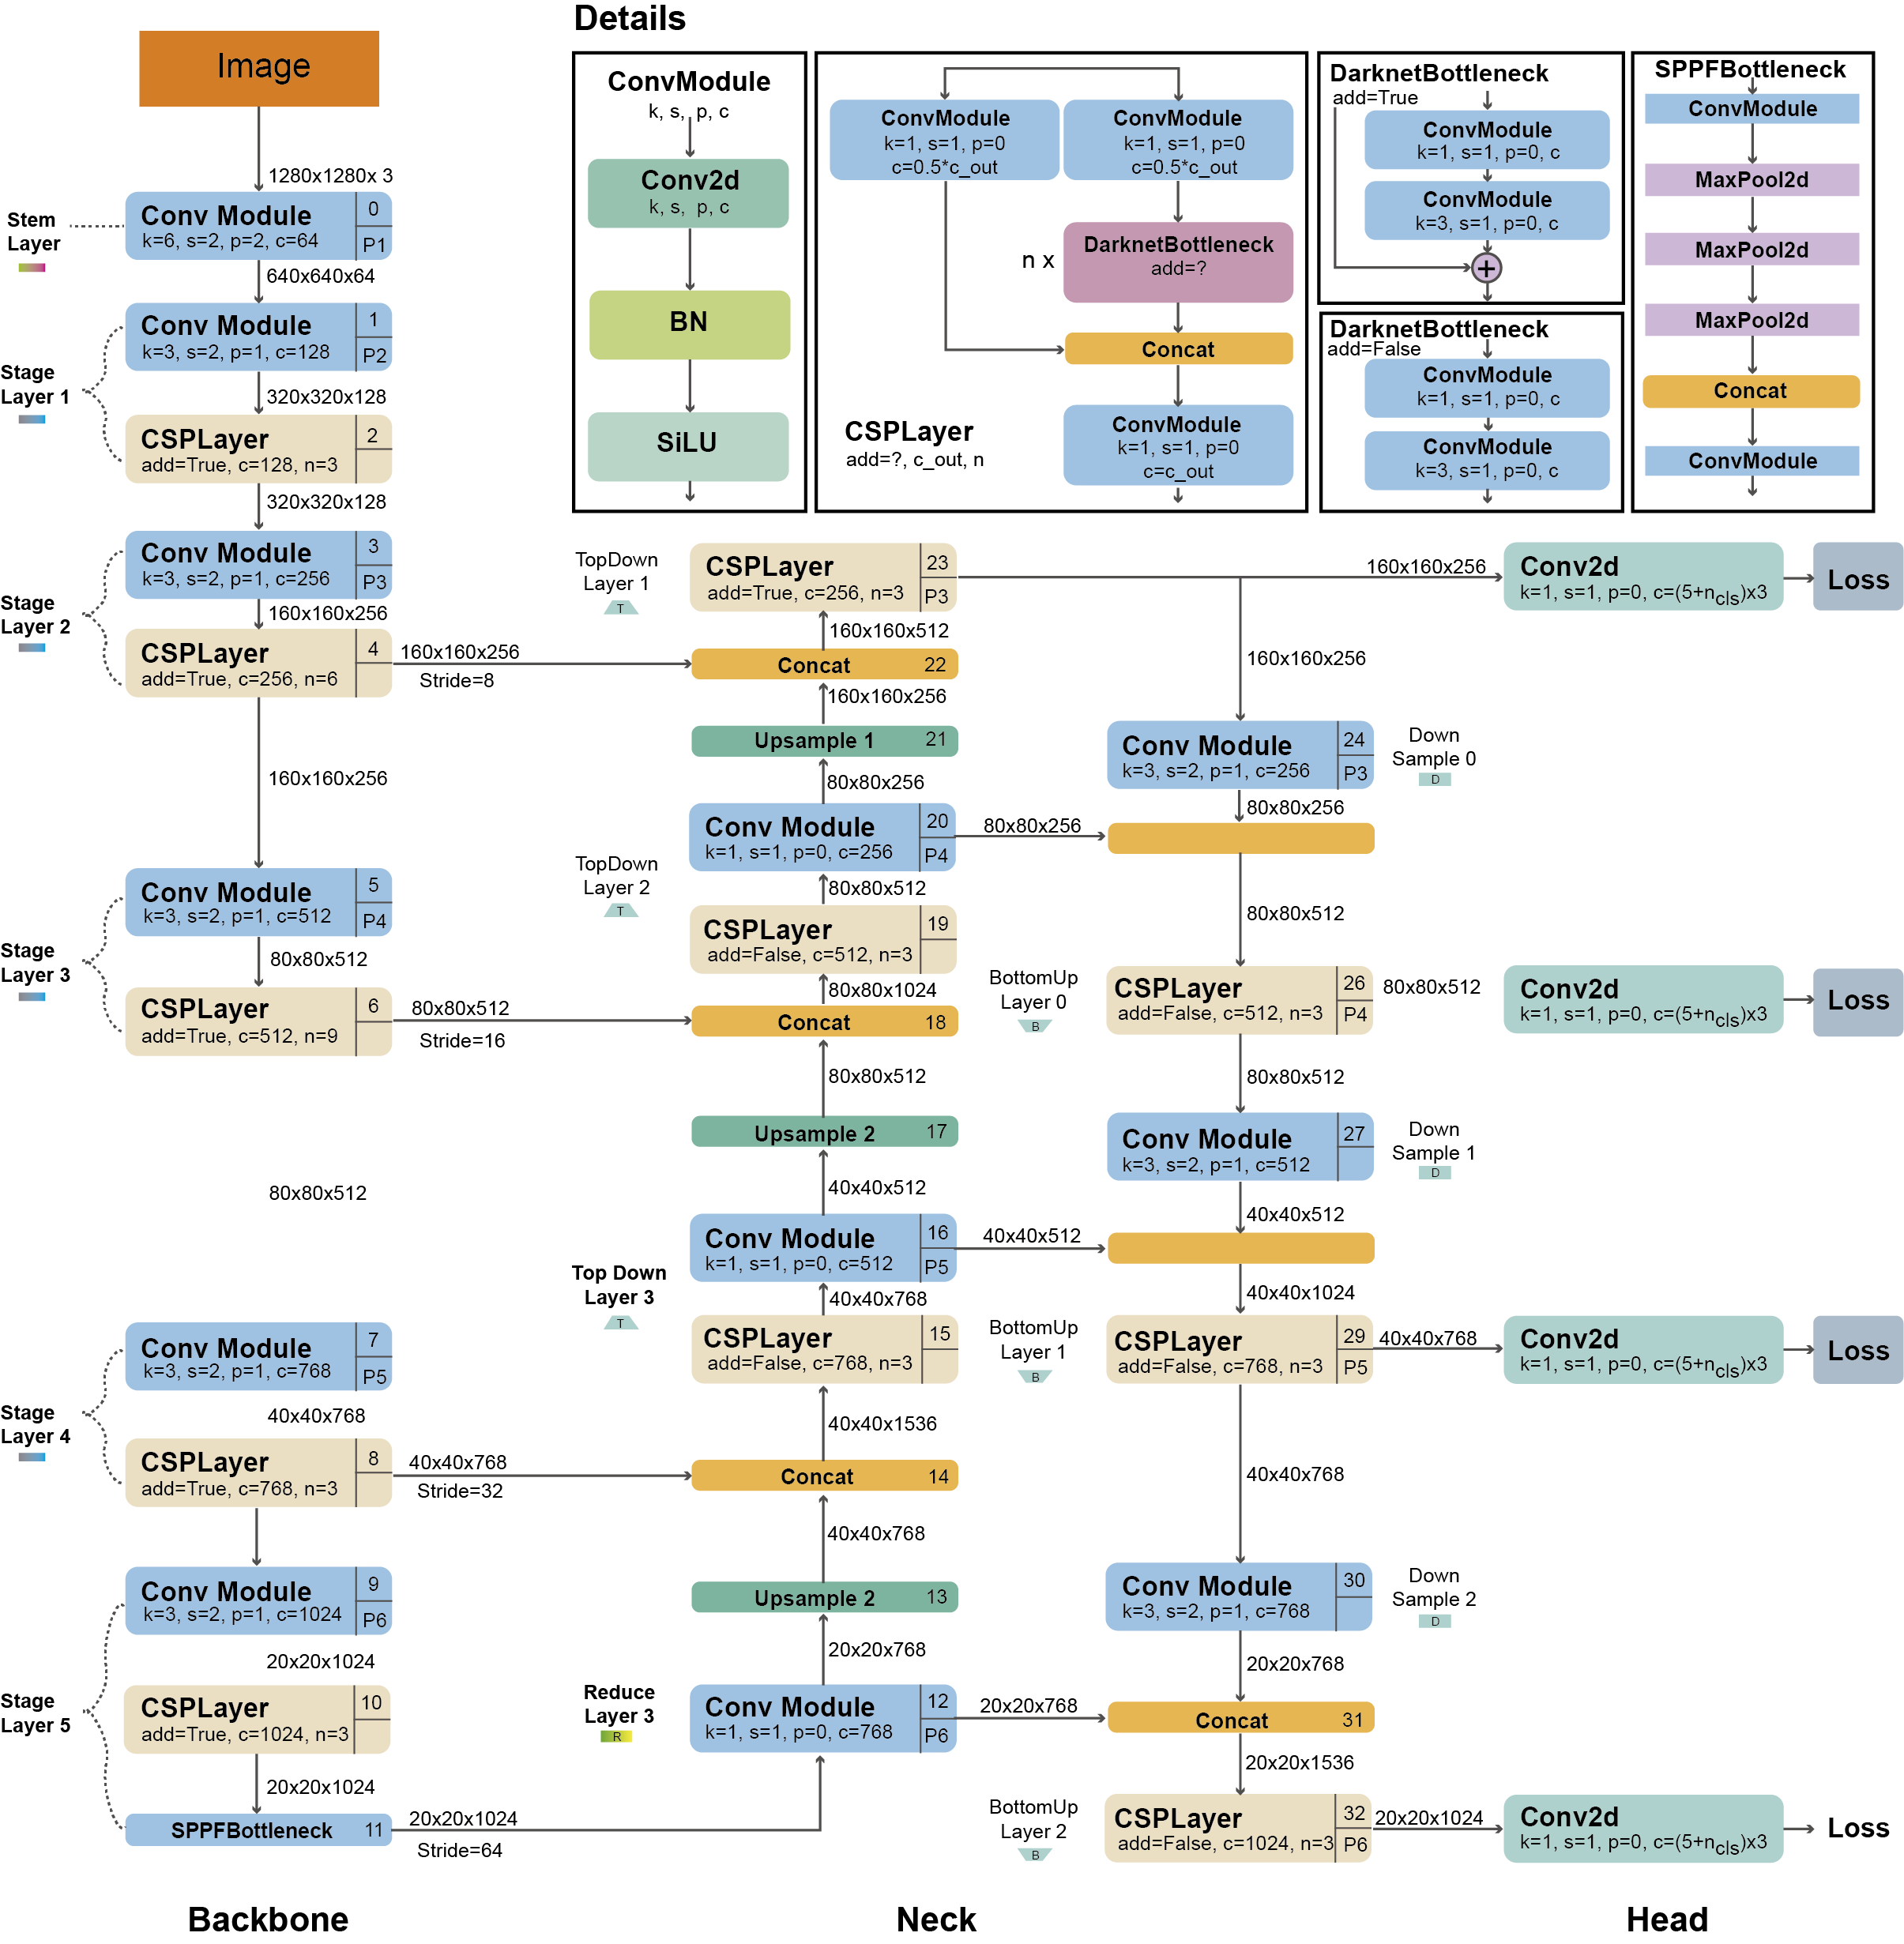
\includegraphics[width=0.88\textwidth]{images/yolov5_architecture.png}
				\caption{YOLOv5 architecture}
				\label{fig:yolov5}
			\end{figure}
		\end{column}
		\begin{column}{0.5\textwidth}
			\begin{figure}[h]
				\centering
				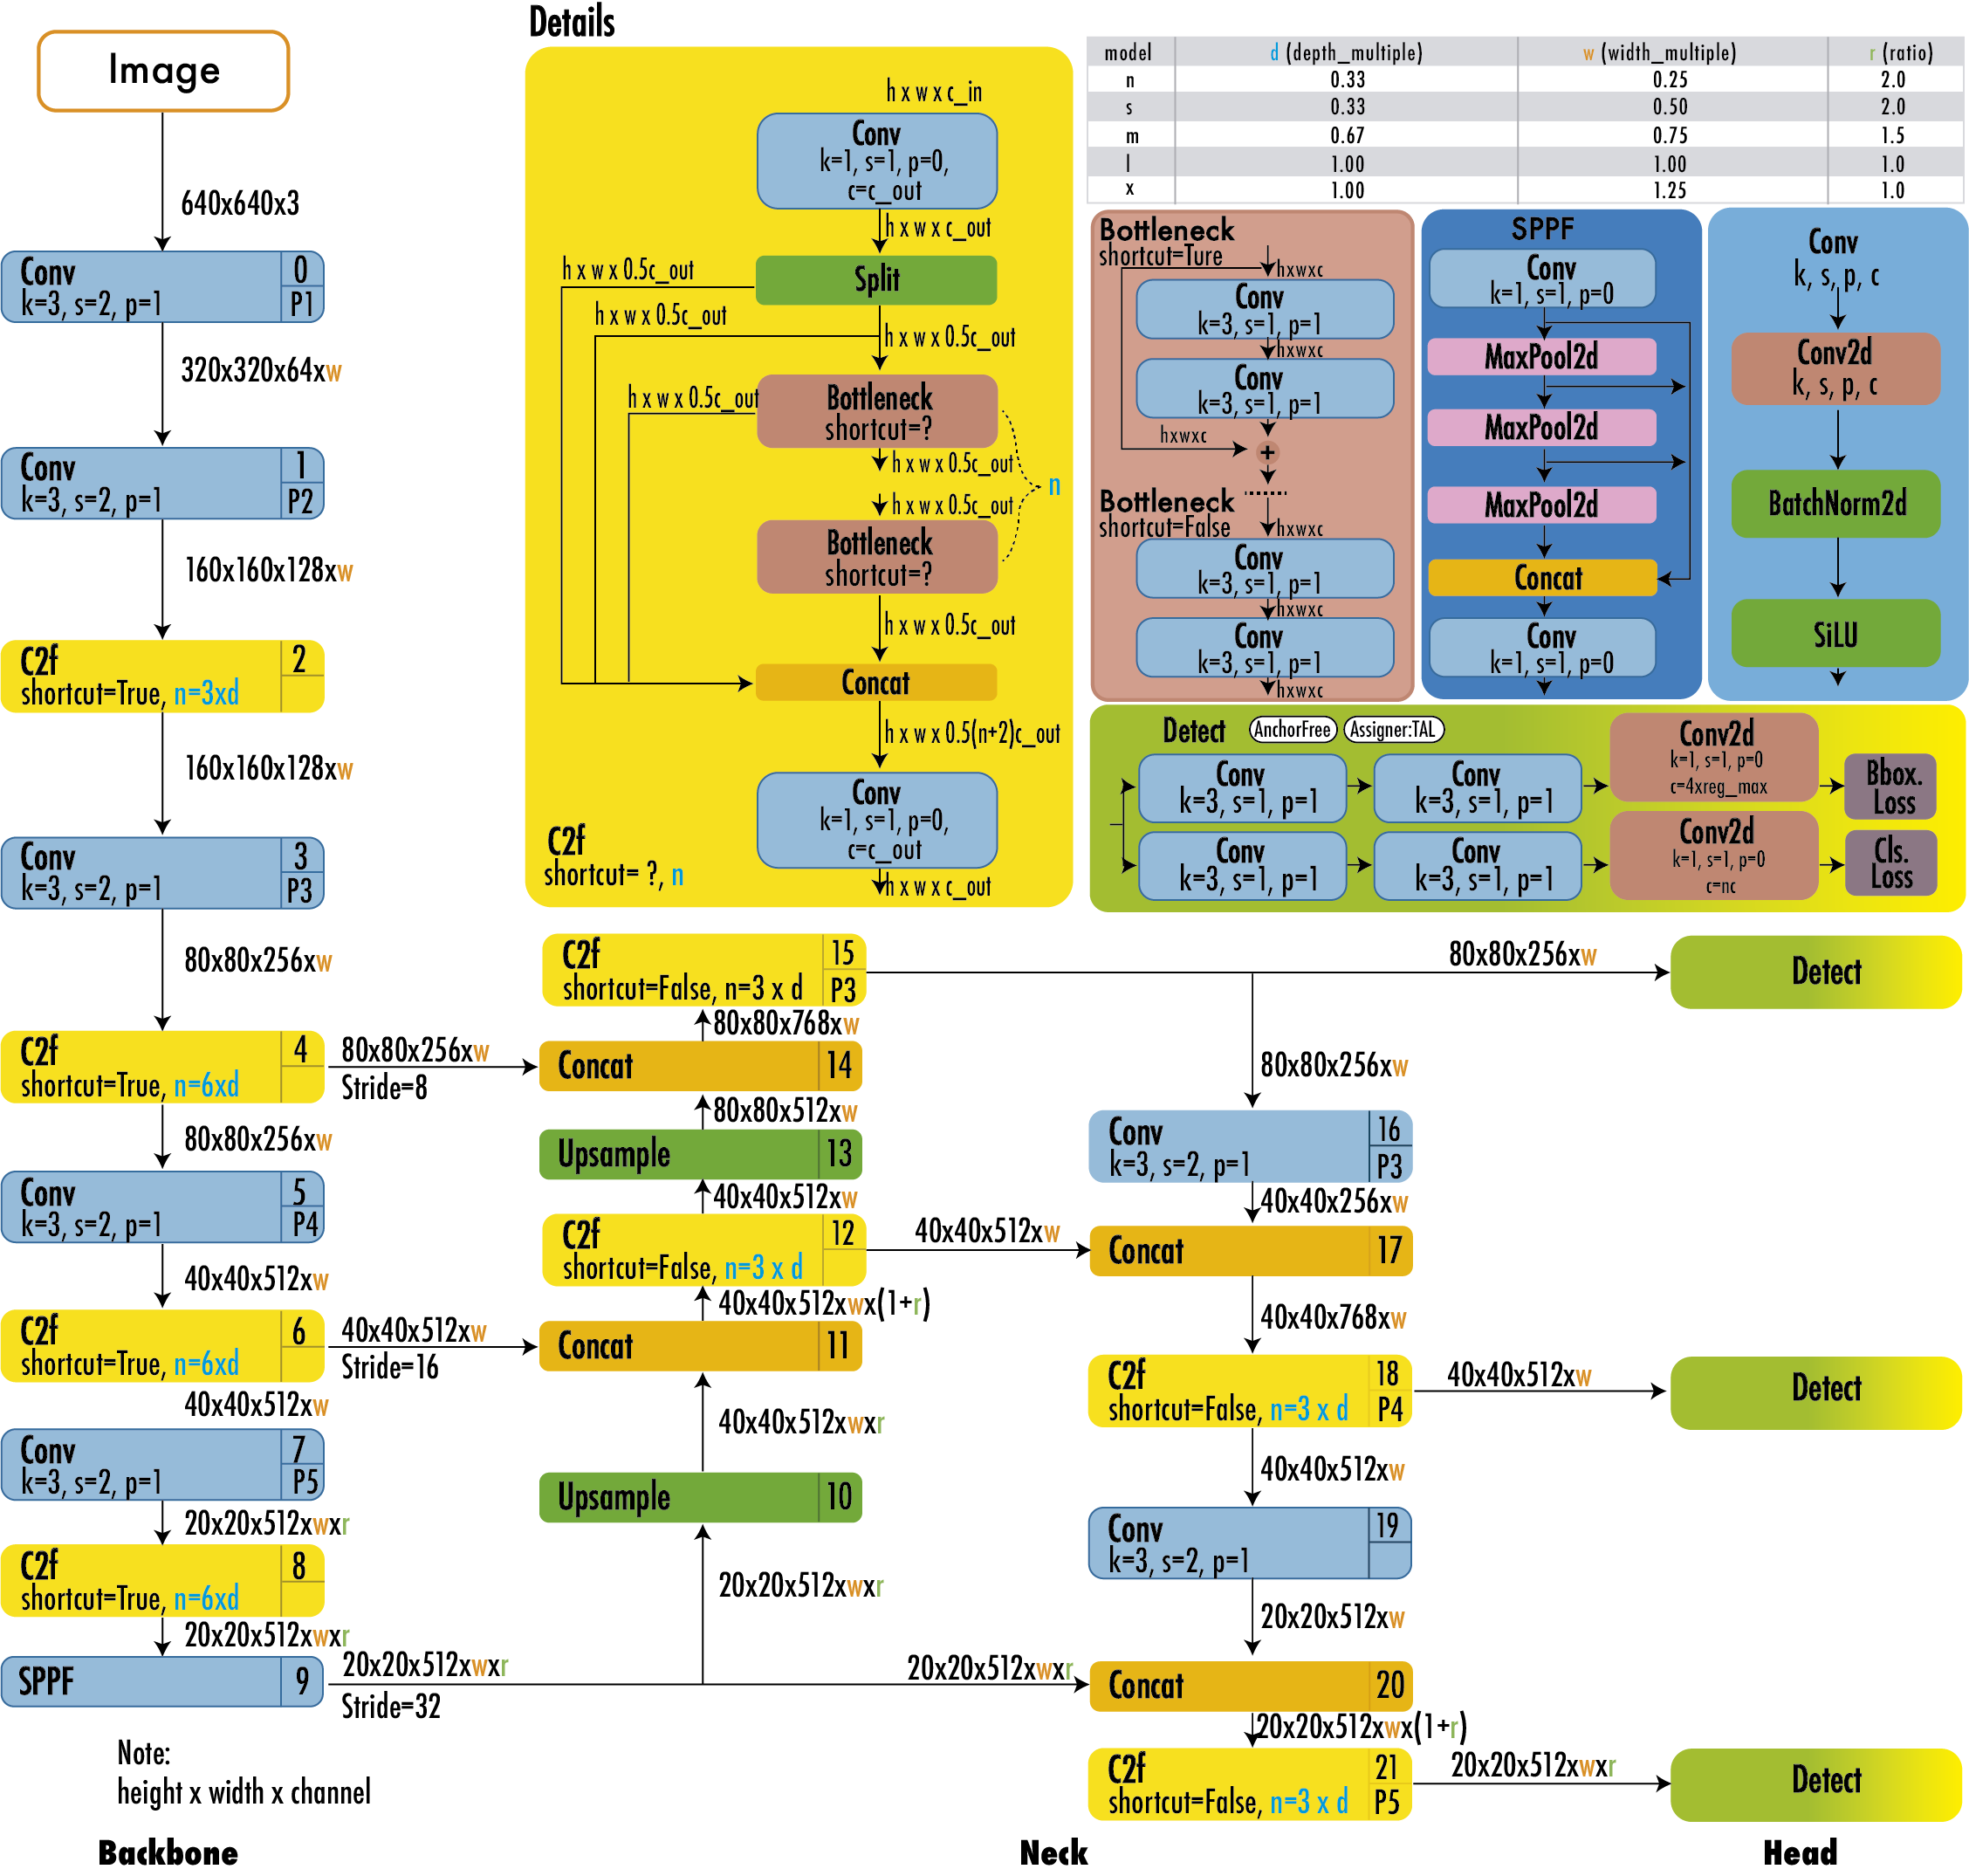
\includegraphics[width=0.85\textwidth]{images/yolov8_architecture.png}
				\caption{YOLOv8 architecture}
				\label{fig:yolov8}
			\end{figure}
		\end{column}
	\end{columns}
\end{frame}

\begin{frame}{Applications}
	\begin{figure}[h]
		\centering
		\includegraphics[width=0.7\textwidth]{images/yolo_apps_.png}
		\caption{Applications on YOLO}
		\label{fig:yolo_apps}
	\end{figure}
\end{frame}

\subsection{Introduction to Combination}
\begin{frame}{Deep Snake}
	\begin{figure}[h]
		\centering
		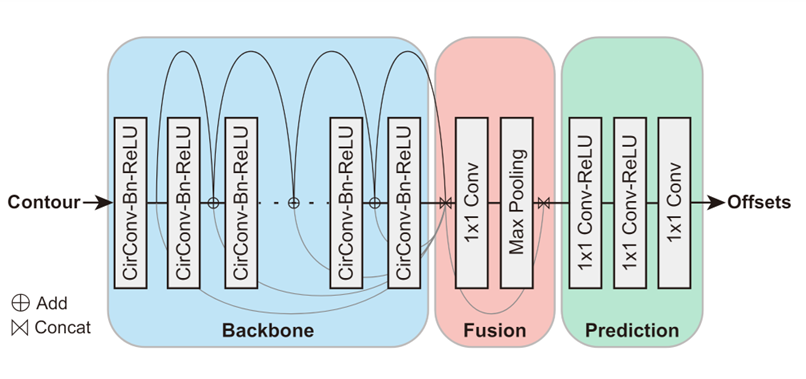
\includegraphics[width=0.7\textwidth]{images/deepsnake_architecture.png}
		\caption{Deep Snake architecture}
		\label{fig:deepsnake_architecture}
	\end{figure}
\end{frame}



\begin{frame}[plain, allowframebreaks, noframenumbering]{Content}
	\tableofcontents
\end{frame}

\section{Experiment}

\subsection{YOLOv8 With EMA and WIoU}
\begin{frame}{Inprovement: Efficient Multi-scale Attention}
	\begin{figure}[h]
		\centering
		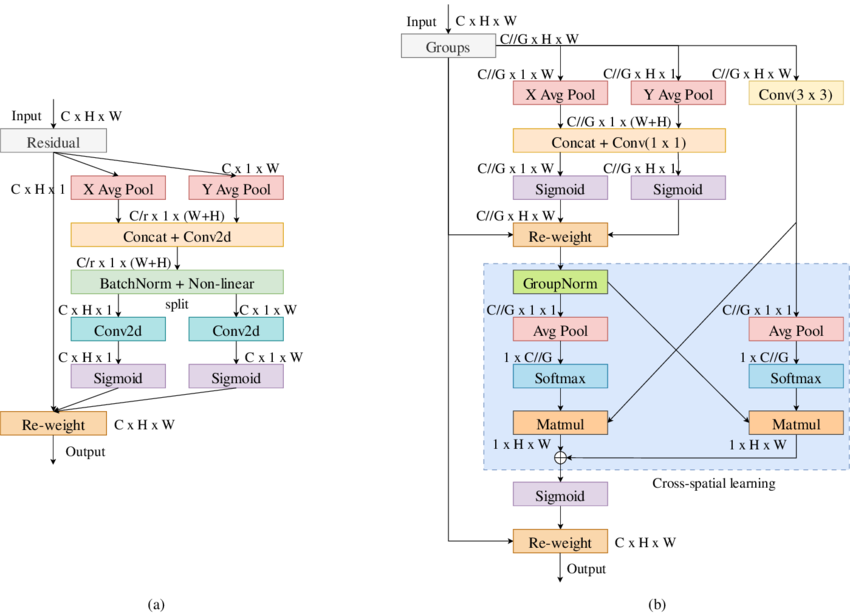
\includegraphics[width=0.65\textwidth]{images/ca_ema.png}
		\caption{Structure of CA and EMA}
		\label{fig:ca_ema}
	\end{figure}
\end{frame}



\begin{frame}{Inprovement: Efficient Multi-scale Attention}
	\begin{block}{Pooling output comparison}
		\begin{columns}
			\begin{column}{0.4\textwidth}
				In coordinate attention(CA), the 1D global average-pooling for encoding information along the horizontal dimension direction in $C$ at height $H$ can be denoted by
				\begin{equation}
					z^H_c(H)=\frac{1}{W}\sum_{0\leq i\leq W} x_c(H,i)
				\end{equation}
				The pooling output in $C$ at width $W$ can be formulated as
				\begin{equation}
					z^W_c(W)=\frac{1}{H}\sum_{0\leq j\leq H}x_c(j,W)
				\end{equation}
			\end{column}
			\begin{column}{0.4\textwidth}
				Efficient multi-scale attention(EMA) employs 2D global average pooling to aggregate cross-spatial information, encoding it into the $1\times 1$ branch output. Outputs of the least branch will be transformed to the correspond dimension shape before the joint activation mechanism of channel features, i.e., $\mathbb{R}^{1\times C//G}_1\times \mathbb{R}^{C//G\times HW}_3$. The 2D global pooling operation is
				\begin{equation}
					z_c=\frac{1}{H\times W}\sum^H_j\sum^W_i x_c(i,j)
				\end{equation}
			\end{column}
		\end{columns}
	\end{block}
\end{frame}

\begin{frame}{Inprovement: Wise-IoU}
	In YOLOv2, we have bounding box regression(BBR) loss expressed as
	\begin{equation}
		\mathcal{L}(\vec{B},\vec{B_{gt}})=\left|\left|\vec{B}-\vec{B_{gt}}\right|\right|
	\end{equation}
	But it cannot shield the inference of the size of the bounding box. So we come up with intersection over union(IoU)
	\begin{equation}
		\mathcal{L}_\text{IoU}=1-\text{IoU}=1-\frac{W_i H_i}{S_i}
	\end{equation}
	In order to prevent circumstances like $W_i=0$ or $H_i$, we add penalty term $\mathcal{R}_i$
	\begin{equation}
		\mathcal{L}_i=\mathcal{L}_\text{IoU}+\mathcal{R}_i
	\end{equation}
	\begin{figure}[h]
		\centering
		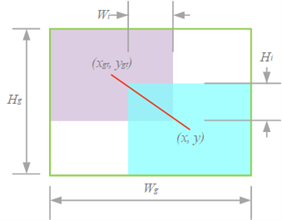
\includegraphics[width=0.21\textwidth]{images/iou.png}
		\caption{An IoU example}
		\label{fig:iou}
	\end{figure}
\end{frame}

\begin{frame}{Inprovement: Wise-IoU}
	\begin{columns}
		\begin{column}{0.5\textwidth}
			\begin{block}{Distance-IoU}
				Consider normalized distance between central points of two bounding boxes
				\begin{equation}
					\mathcal{R}_\text{DIoU}=\frac{\left(x-x_{g t}\right)^2+\left(y-y_{g t}\right)^2}{W_g^2+H_g^2}
				\end{equation}
			\end{block}
		\end{column}
		\pause
		\begin{column}{0.5\textwidth}
			\begin{block}{Complete-IoU}
				Add the consideration of aspect ratio
				\begin{equation}
					\mathcal{R}_\text{CIoU}=\mathcal{R}_\text{DIoU}+\alpha v,\alpha=\frac{v}{\mathcal{L}_\text{IoU}+v}
				\end{equation}
			\end{block}
		\end{column}
	\end{columns}
\end{frame}

\begin{frame}{Inprovement: Wise-IoU}
	\begin{columns}
		\begin{column}{0.45\textwidth}
			\begin{block}{Efficient-IoU}
				Increase the punishment for distance metric
				\begin{equation}
					\mathcal{R}_\text{EIoU}=\mathcal{R}_\text{DIoU}+\frac{\left(x-x_{g t}\right)^2}{W_g^2}+\frac{\left(y-y_{g t}\right)^2}{H_g^2}
				\end{equation}
			\end{block}
		\end{column}
		\pause
		\begin{column}{0.55\textwidth}
			\begin{block}{Scylla-IoU}
				We define angle cost as
				\begin{equation}
					\Lambda=\sin \left(2 \sin ^{-1} \frac{\min \left(\left|x-x_{g t}\right|,\left|y-y_{g t}\right|\right)}{\sqrt{\left(x-x_{g t}\right)^2+\left(y-y_{g t}\right)^2}+\varepsilon}\right)
				\end{equation}
				Then the distance cost comes to be
				\begin{equation}
					\Delta=\frac{1}{2} \sum_{t=w, h}\left(1-e^{-\gamma \rho_t}\right), \gamma=2-\Lambda
				\end{equation}
				Therefore, we have
				\begin{equation}
					\mathcal{R}_\text{SIoU}=\Delta+\Sigma
				\end{equation}
			\end{block}
		\end{column}
	\end{columns}
\end{frame}

\begin{frame}{Inprovement: Wise-IoU}
	\begin{block}{Wise-IoU}
		Based on SIoU and EIou, we reconsider low-quality examples and geometric factors, and construct Wise-IoU with 2 layers of attention mechanism
		\begin{equation}
			\mathcal{L}_\text{WIoU}=\mathcal{R}_\text{WIoU}\mathcal{L}_\text{IoU}
		\end{equation}
		where
		\begin{equation}
			\mathcal{R}_\text{WIoU}=\exp\left(\frac{(x-x_{gt})^2+(y-y_{gt})^2}{(W^2_g+H^2_g)^*}\right)
		\end{equation}
		$\mathcal{R}_\text{WIoU}\in [1,e)$ which will significantly amplify $\mathcal{L}_\text{IoU}$ of the ordinary-quality anchor box. $\mathcal{L}_\text{IoU}\in [0,1]$, which will significantly reduce $\mathcal{R}_\text{WIoU}$ of the high-quality anchor box and its focus on the distance between central points when the anchor box coincides well with the target box.\\
		Superscript $*$ indicates $W_g,H_g$ are detached from the computational graph.
	\end{block}
\end{frame}

\begin{frame}{Experiment: Where to add EMA?}
	\begin{figure}[h]
		\centering
		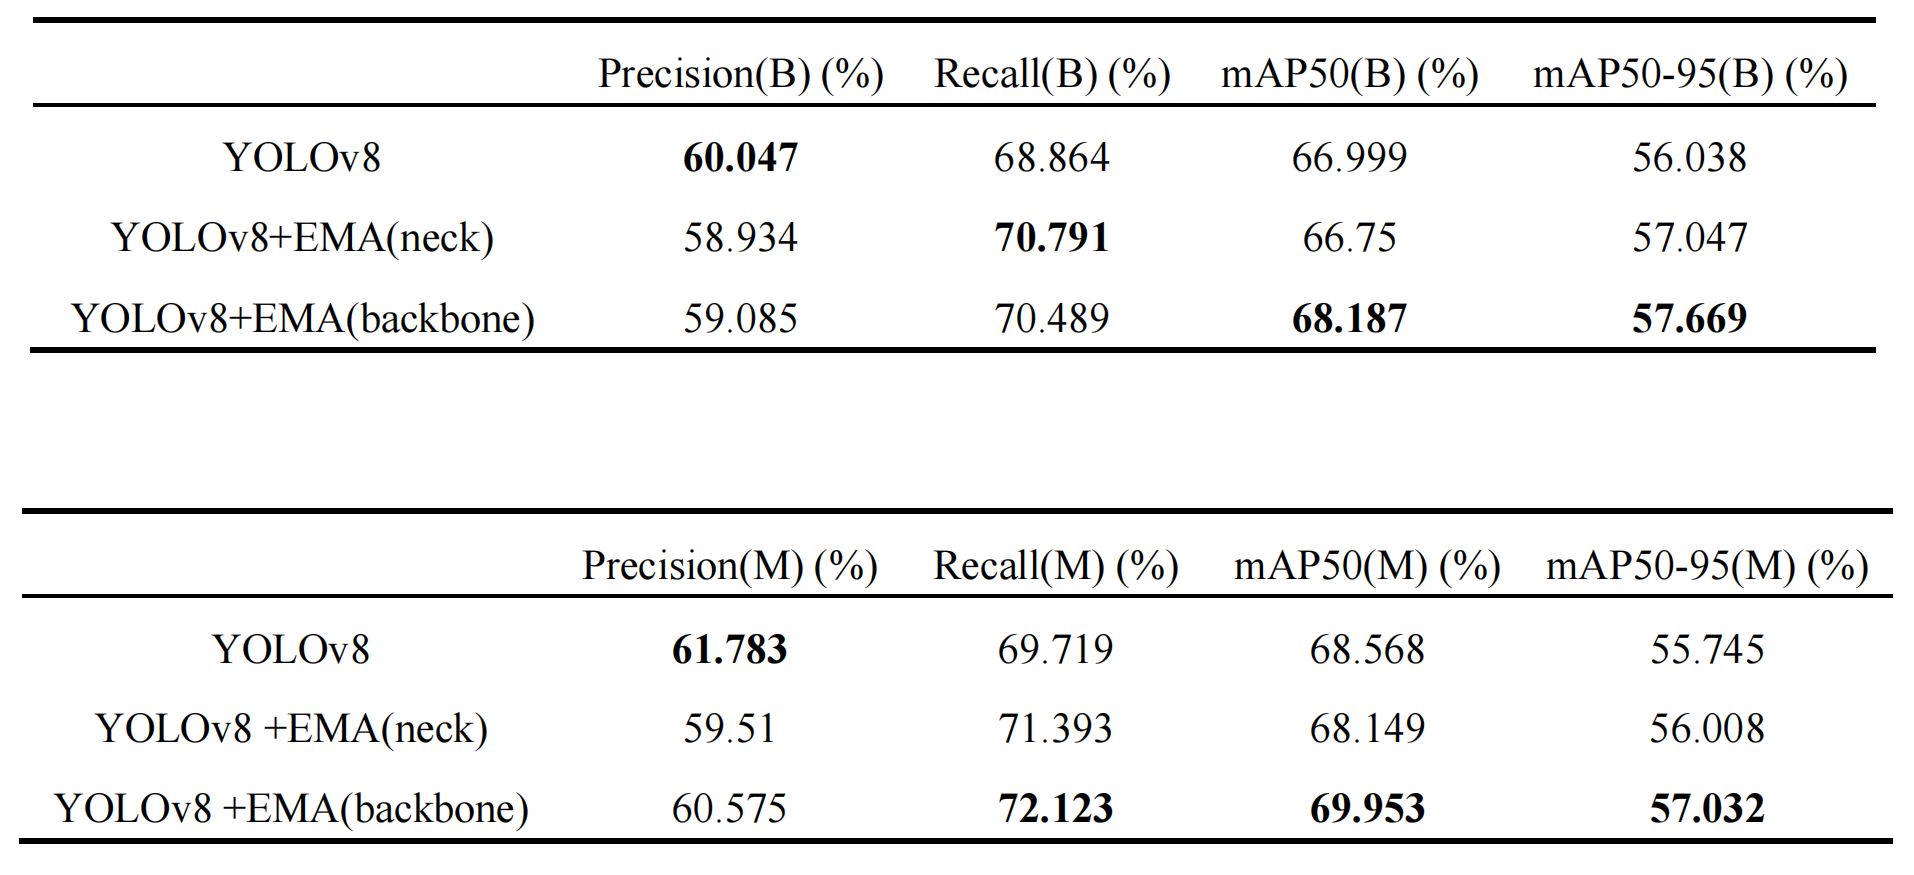
\includegraphics[width=\textwidth]{images/ema_add.png}
		\caption*{}
	\end{figure}
\end{frame}

\begin{frame}{Experiment: How's the combination?}
	\begin{figure}[h]
		\centering
		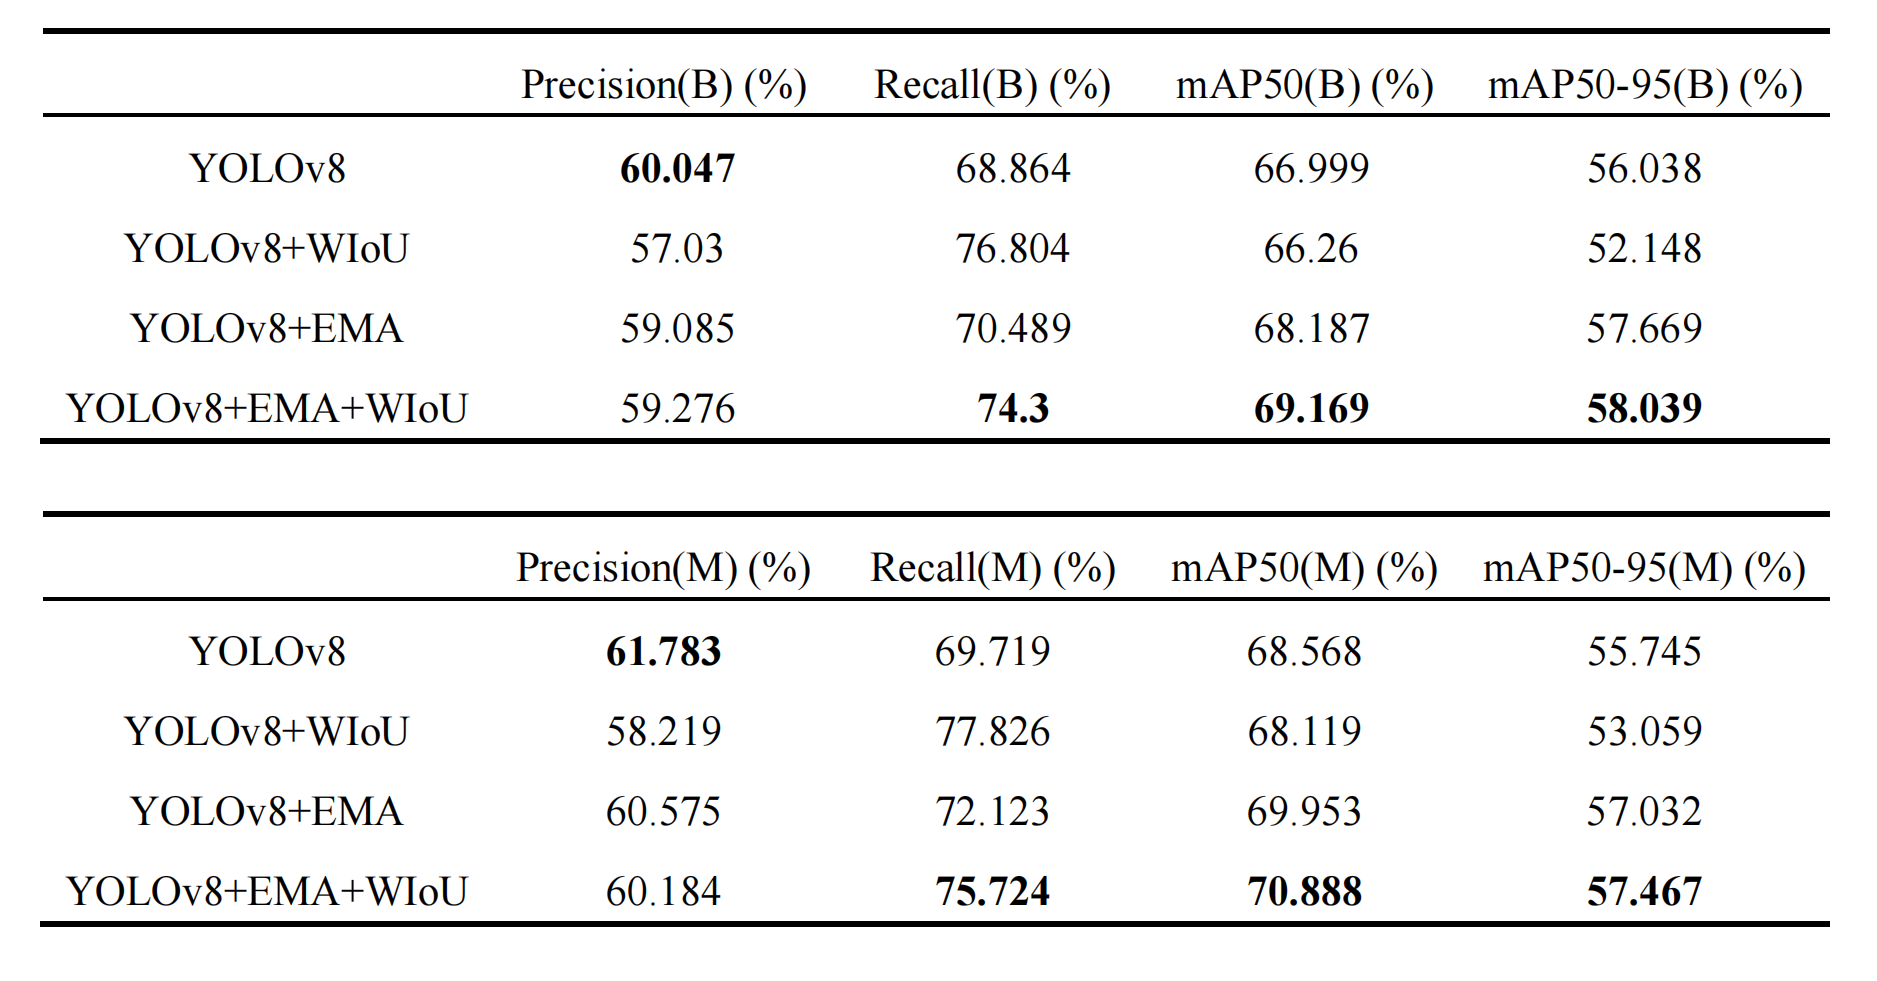
\includegraphics[width=\textwidth]{images/improve_combination.png}
		\caption*{}
	\end{figure}
\end{frame}

\begin{frame}{Assessment: EMA and WIoU}
	\begin{figure}[h]
		\centering
		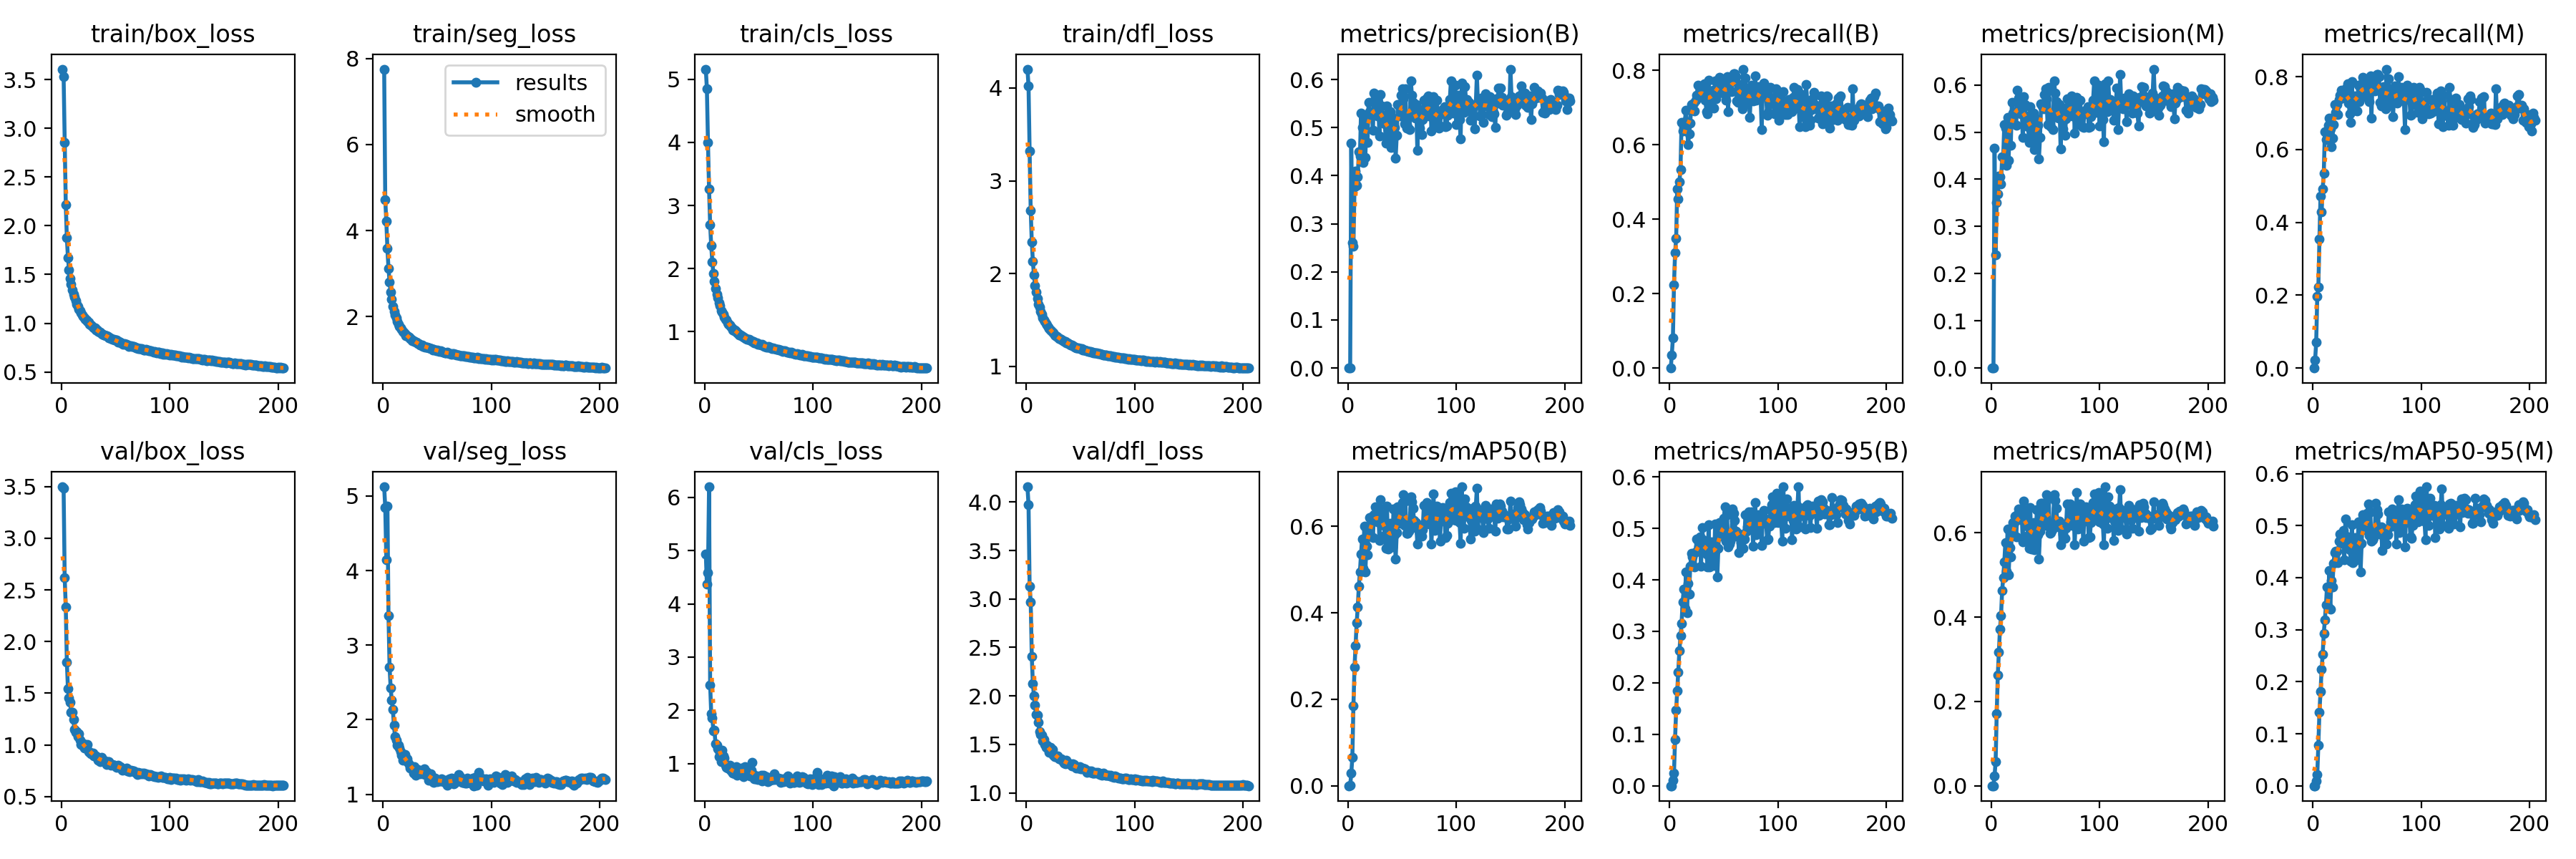
\includegraphics[width=\textwidth]{images/loss_1.png}
		\caption{Results}
		\label{fig:loss1}
	\end{figure}
\end{frame}

\begin{frame}{Assessment: EMA and WIoU}
	\begin{columns}
		\begin{column}{0.5\textwidth}
			\begin{figure}[h]
				\centering
				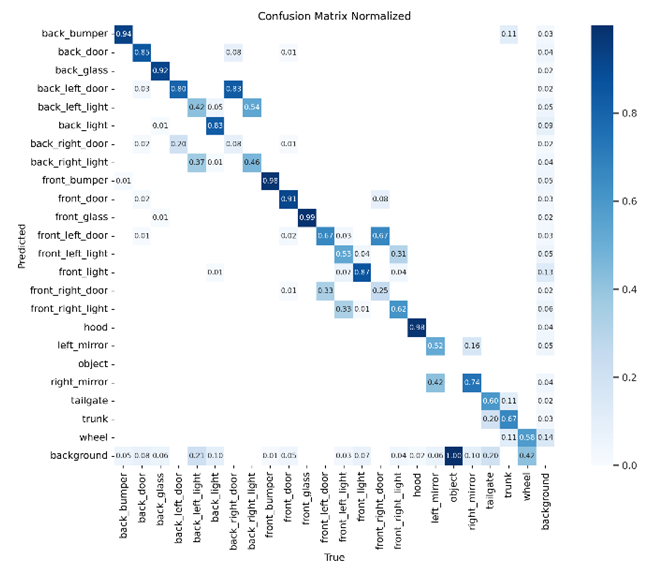
\includegraphics[width=0.87\textwidth]{images/confusion_origin.png}
				\caption{Original YOLOv8 confusion matrix}
				\label{fig:confusion_origin}
			\end{figure}
		\end{column}
		\begin{column}{0.5\textwidth}
			\begin{figure}[h]
				\centering
				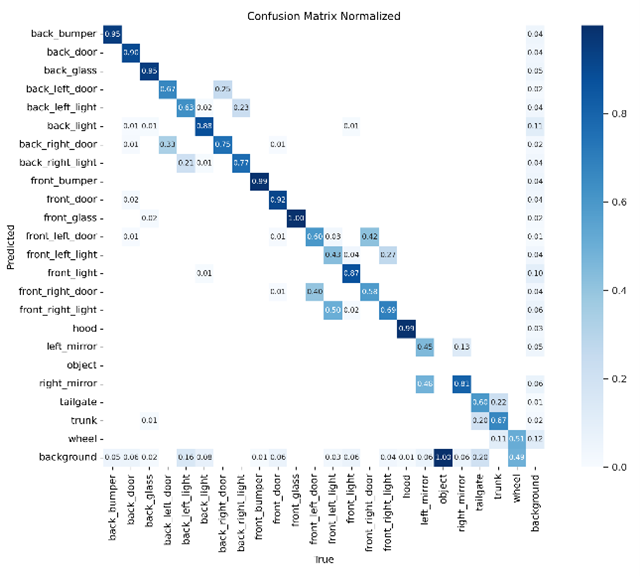
\includegraphics[width=0.85\textwidth]{images/confusion_improve.png}
				\caption{Improved YOLOv8 confusion matrix}
				\label{fig:confusion_improve}
			\end{figure}
		\end{column}
	\end{columns}
\end{frame}

\begin{frame}{Results: EMA and WIoU}
	\begin{columns}
		\begin{column}{0.5\textwidth}
			\begin{figure}[h]
				\centering
				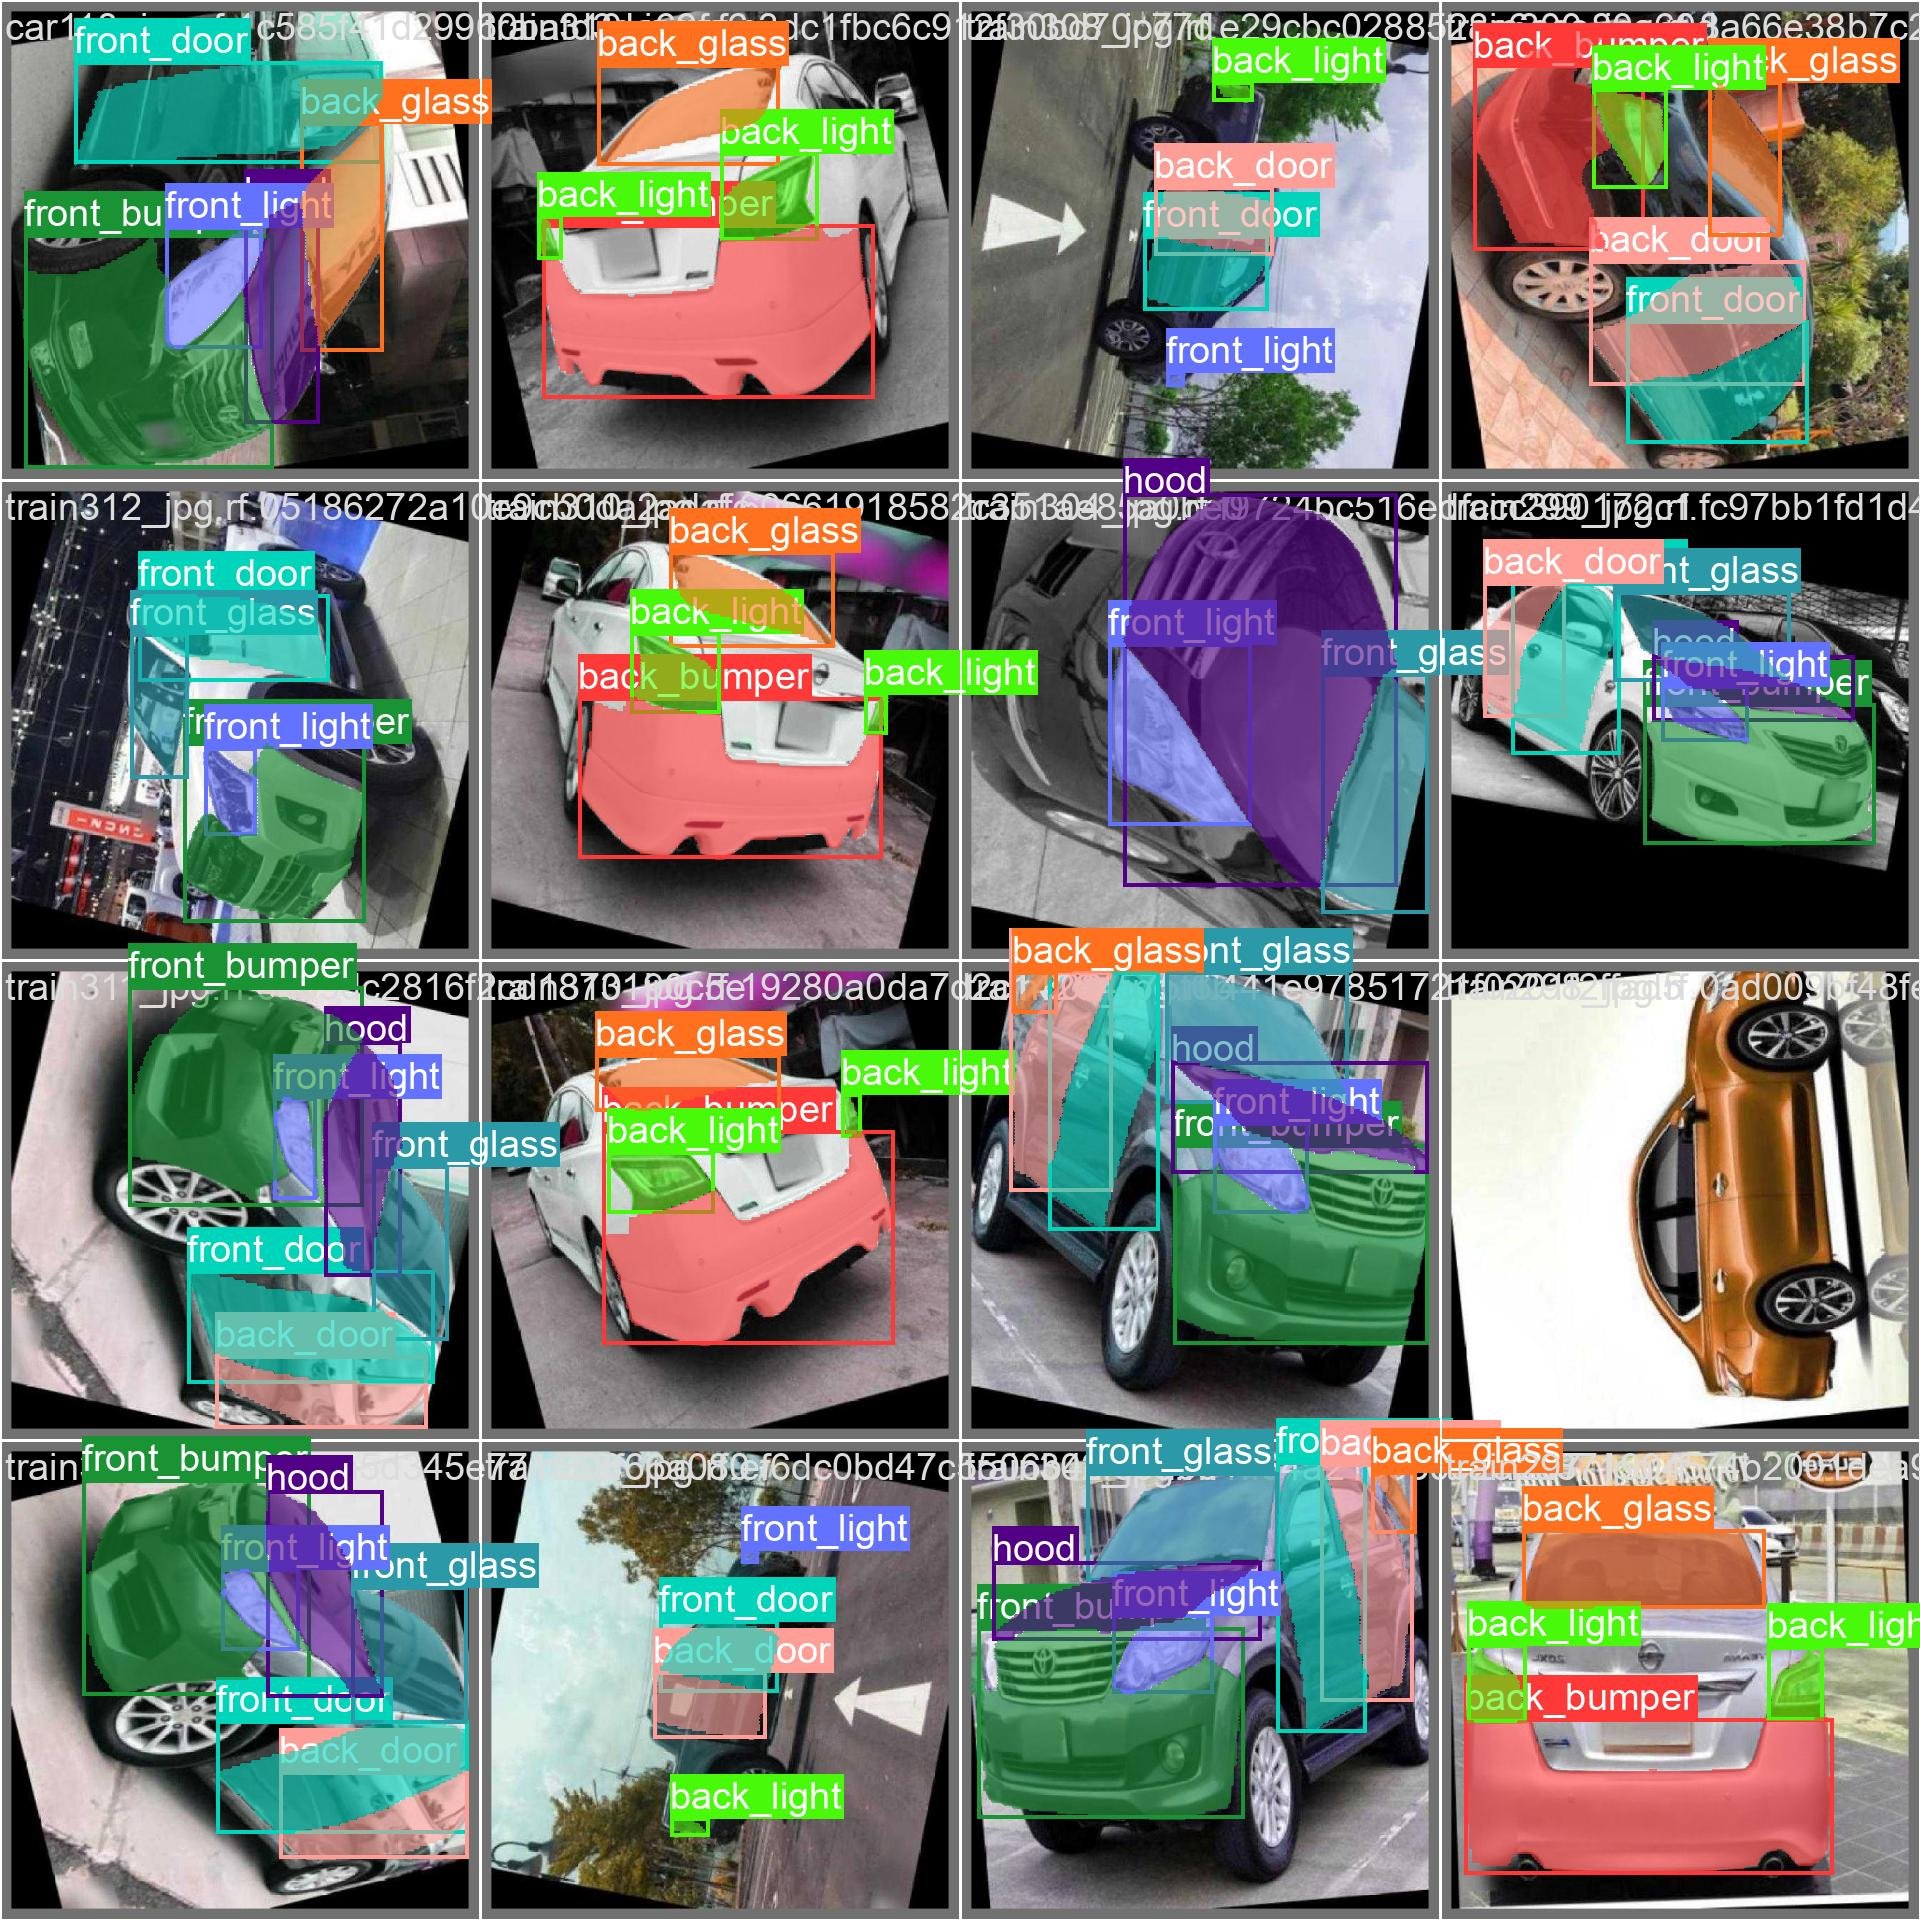
\includegraphics[width=0.7\columnwidth]{images/origin.jpg}
				\caption{Original labels}
%				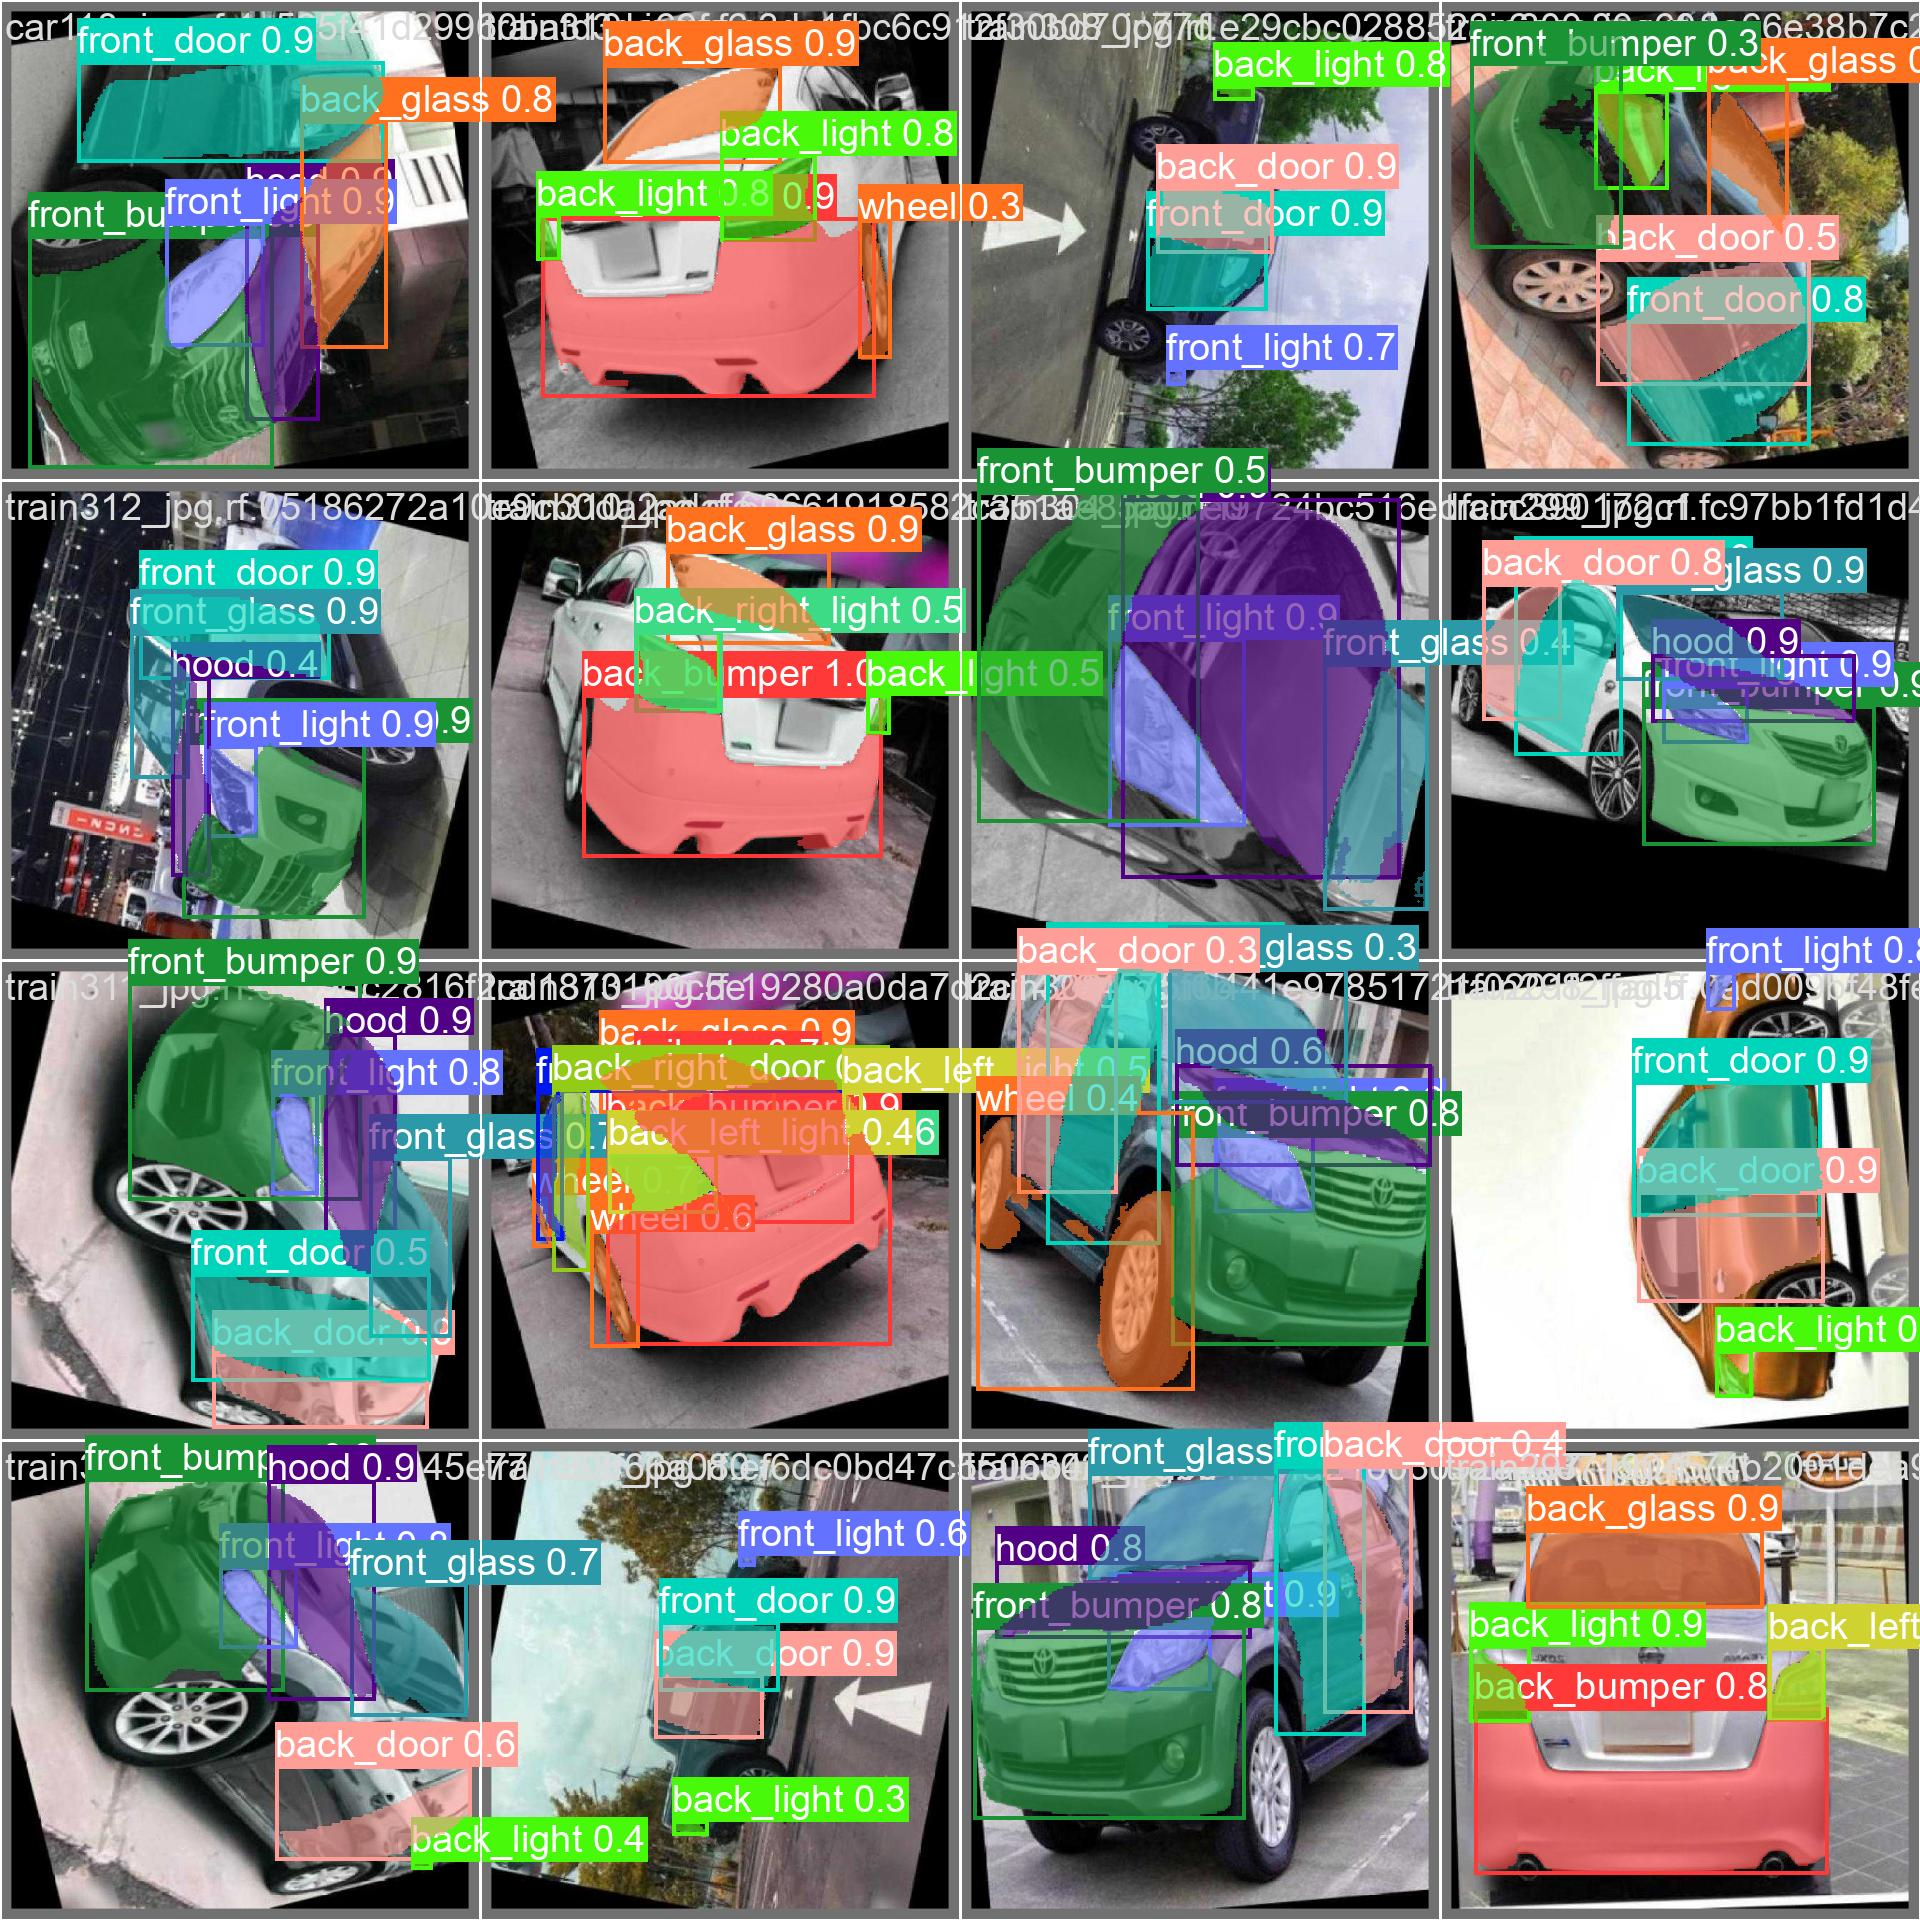
\includegraphics[width=0.45\columnwidth]{images/yolov8.jpg}
%				\caption{YOLOv8 segmentation}
			\end{figure}
		\end{column}
		\begin{column}{0.5\textwidth}
			\begin{figure}[h]
%				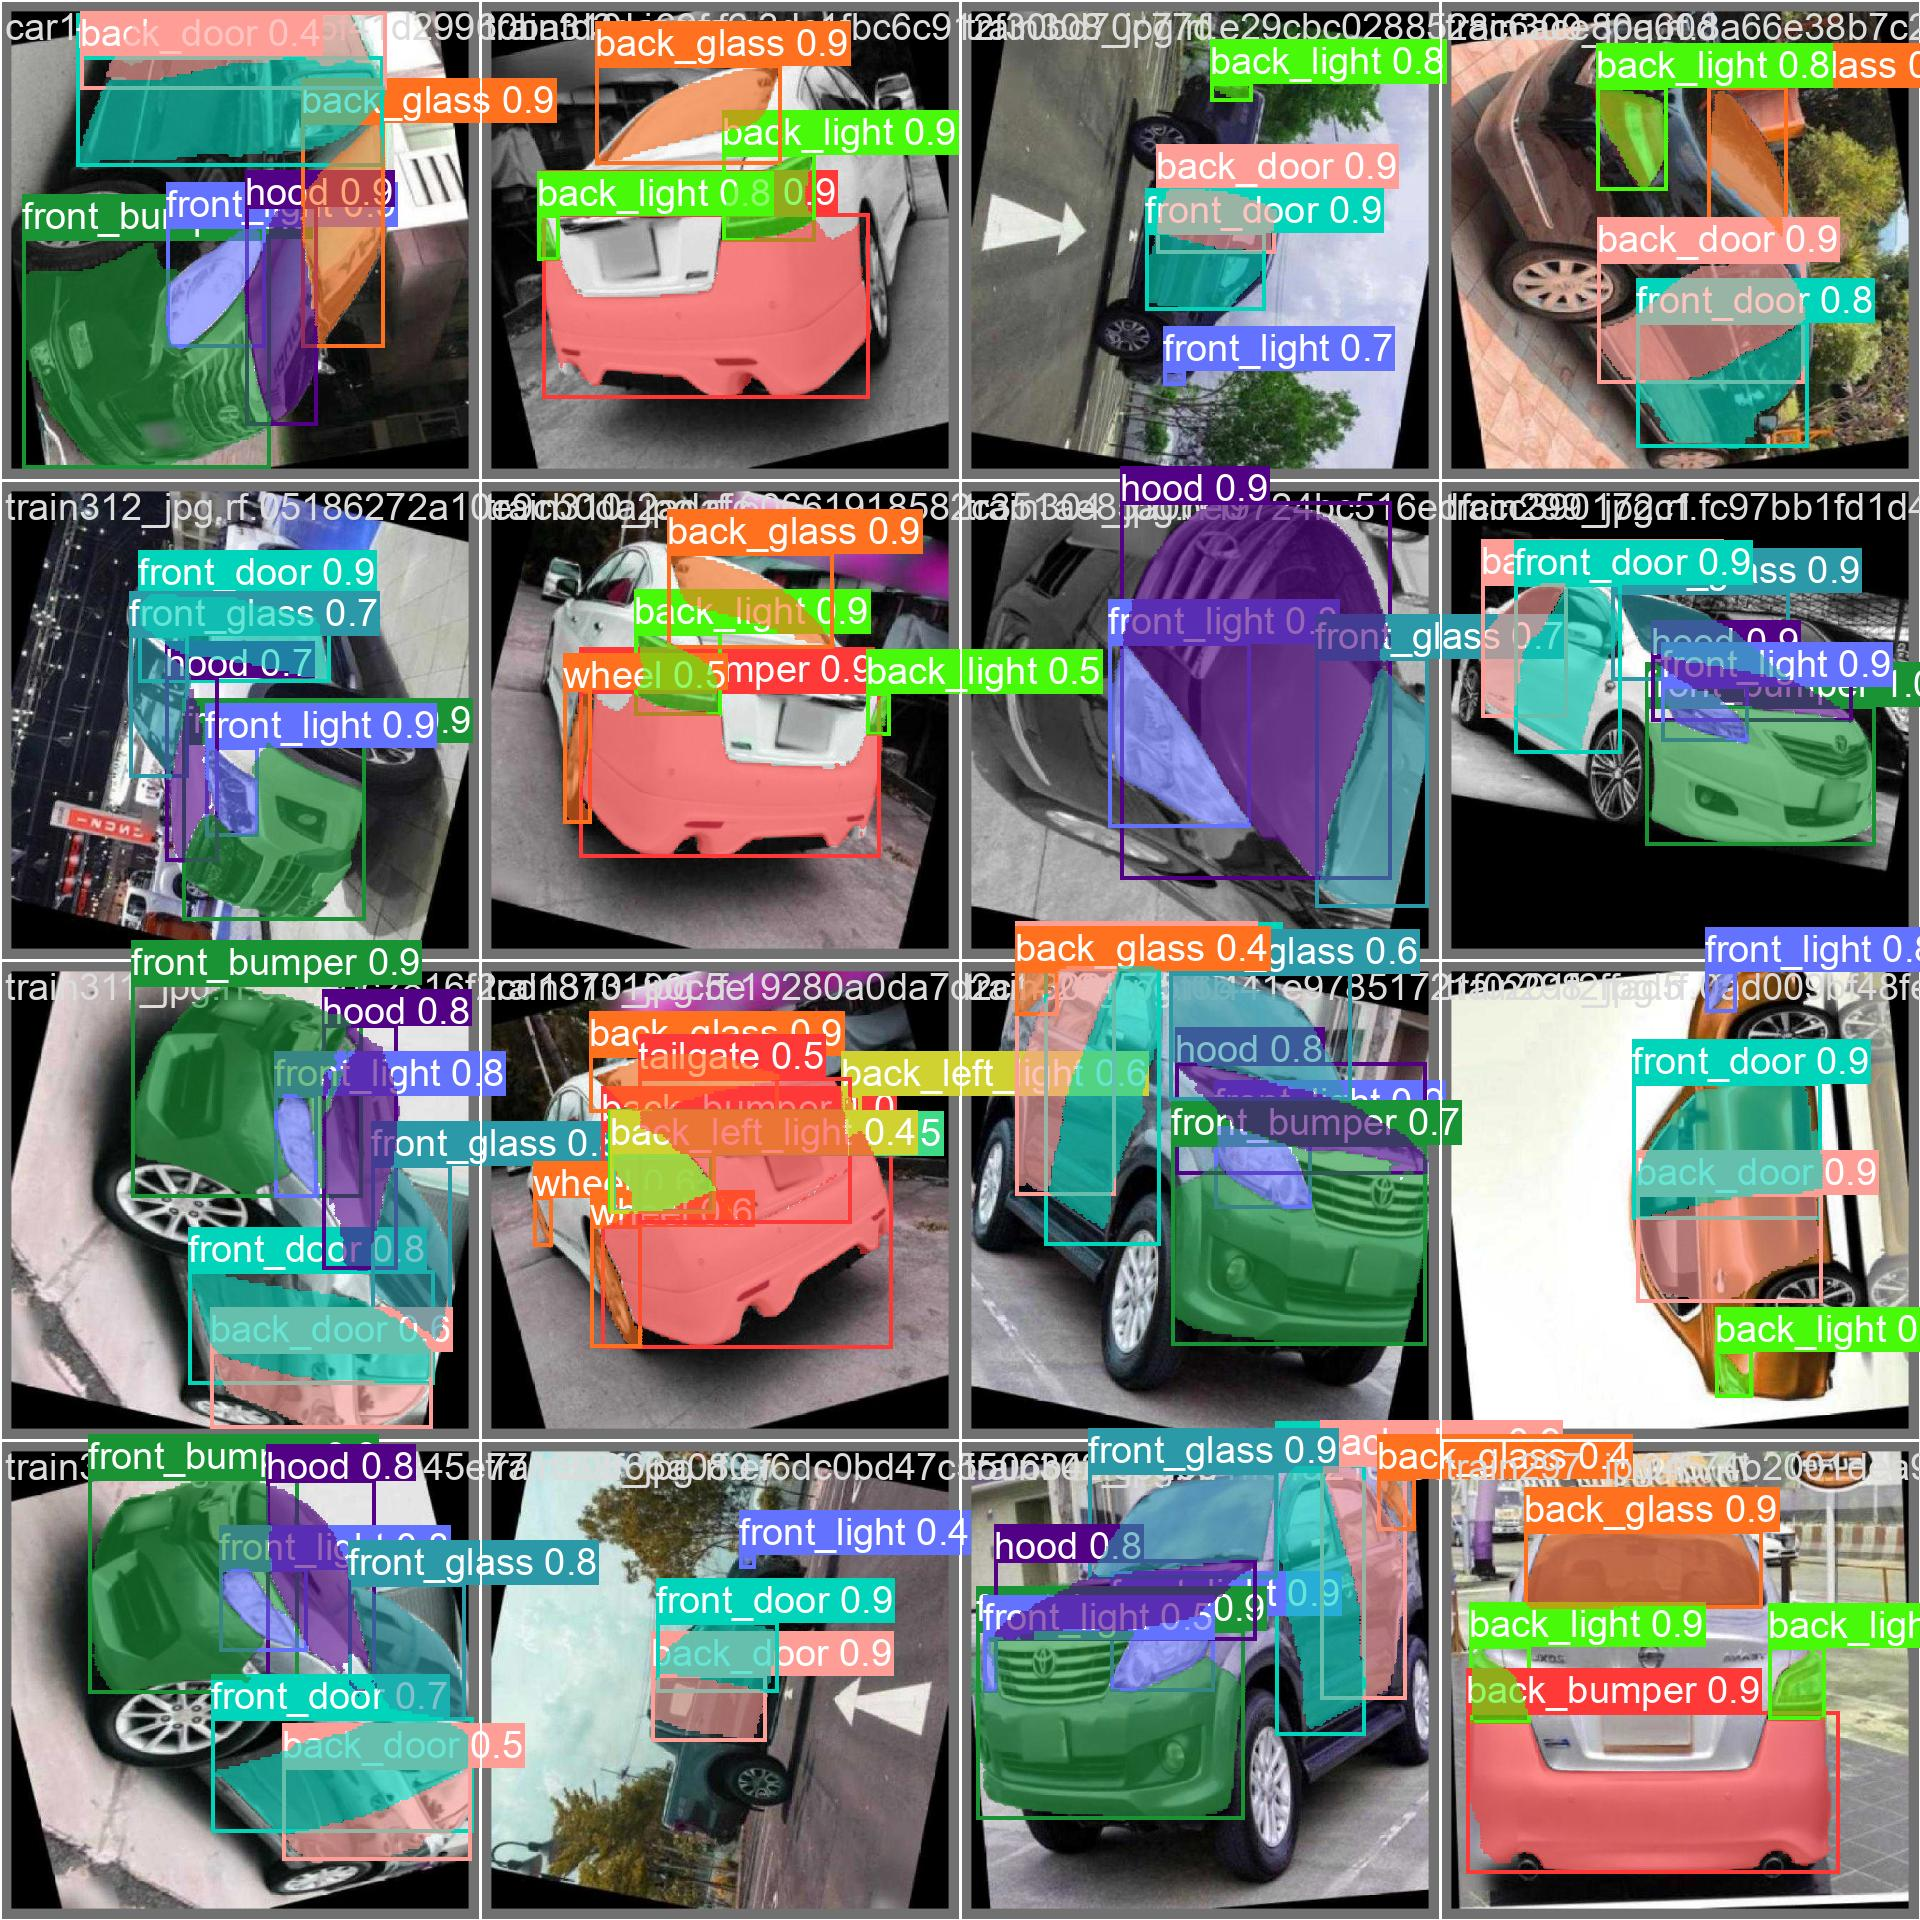
\includegraphics[width=0.45\columnwidth]{images/ema_backbone.jpg}
%				\caption{YOLOv8 with EMA segmentation}
				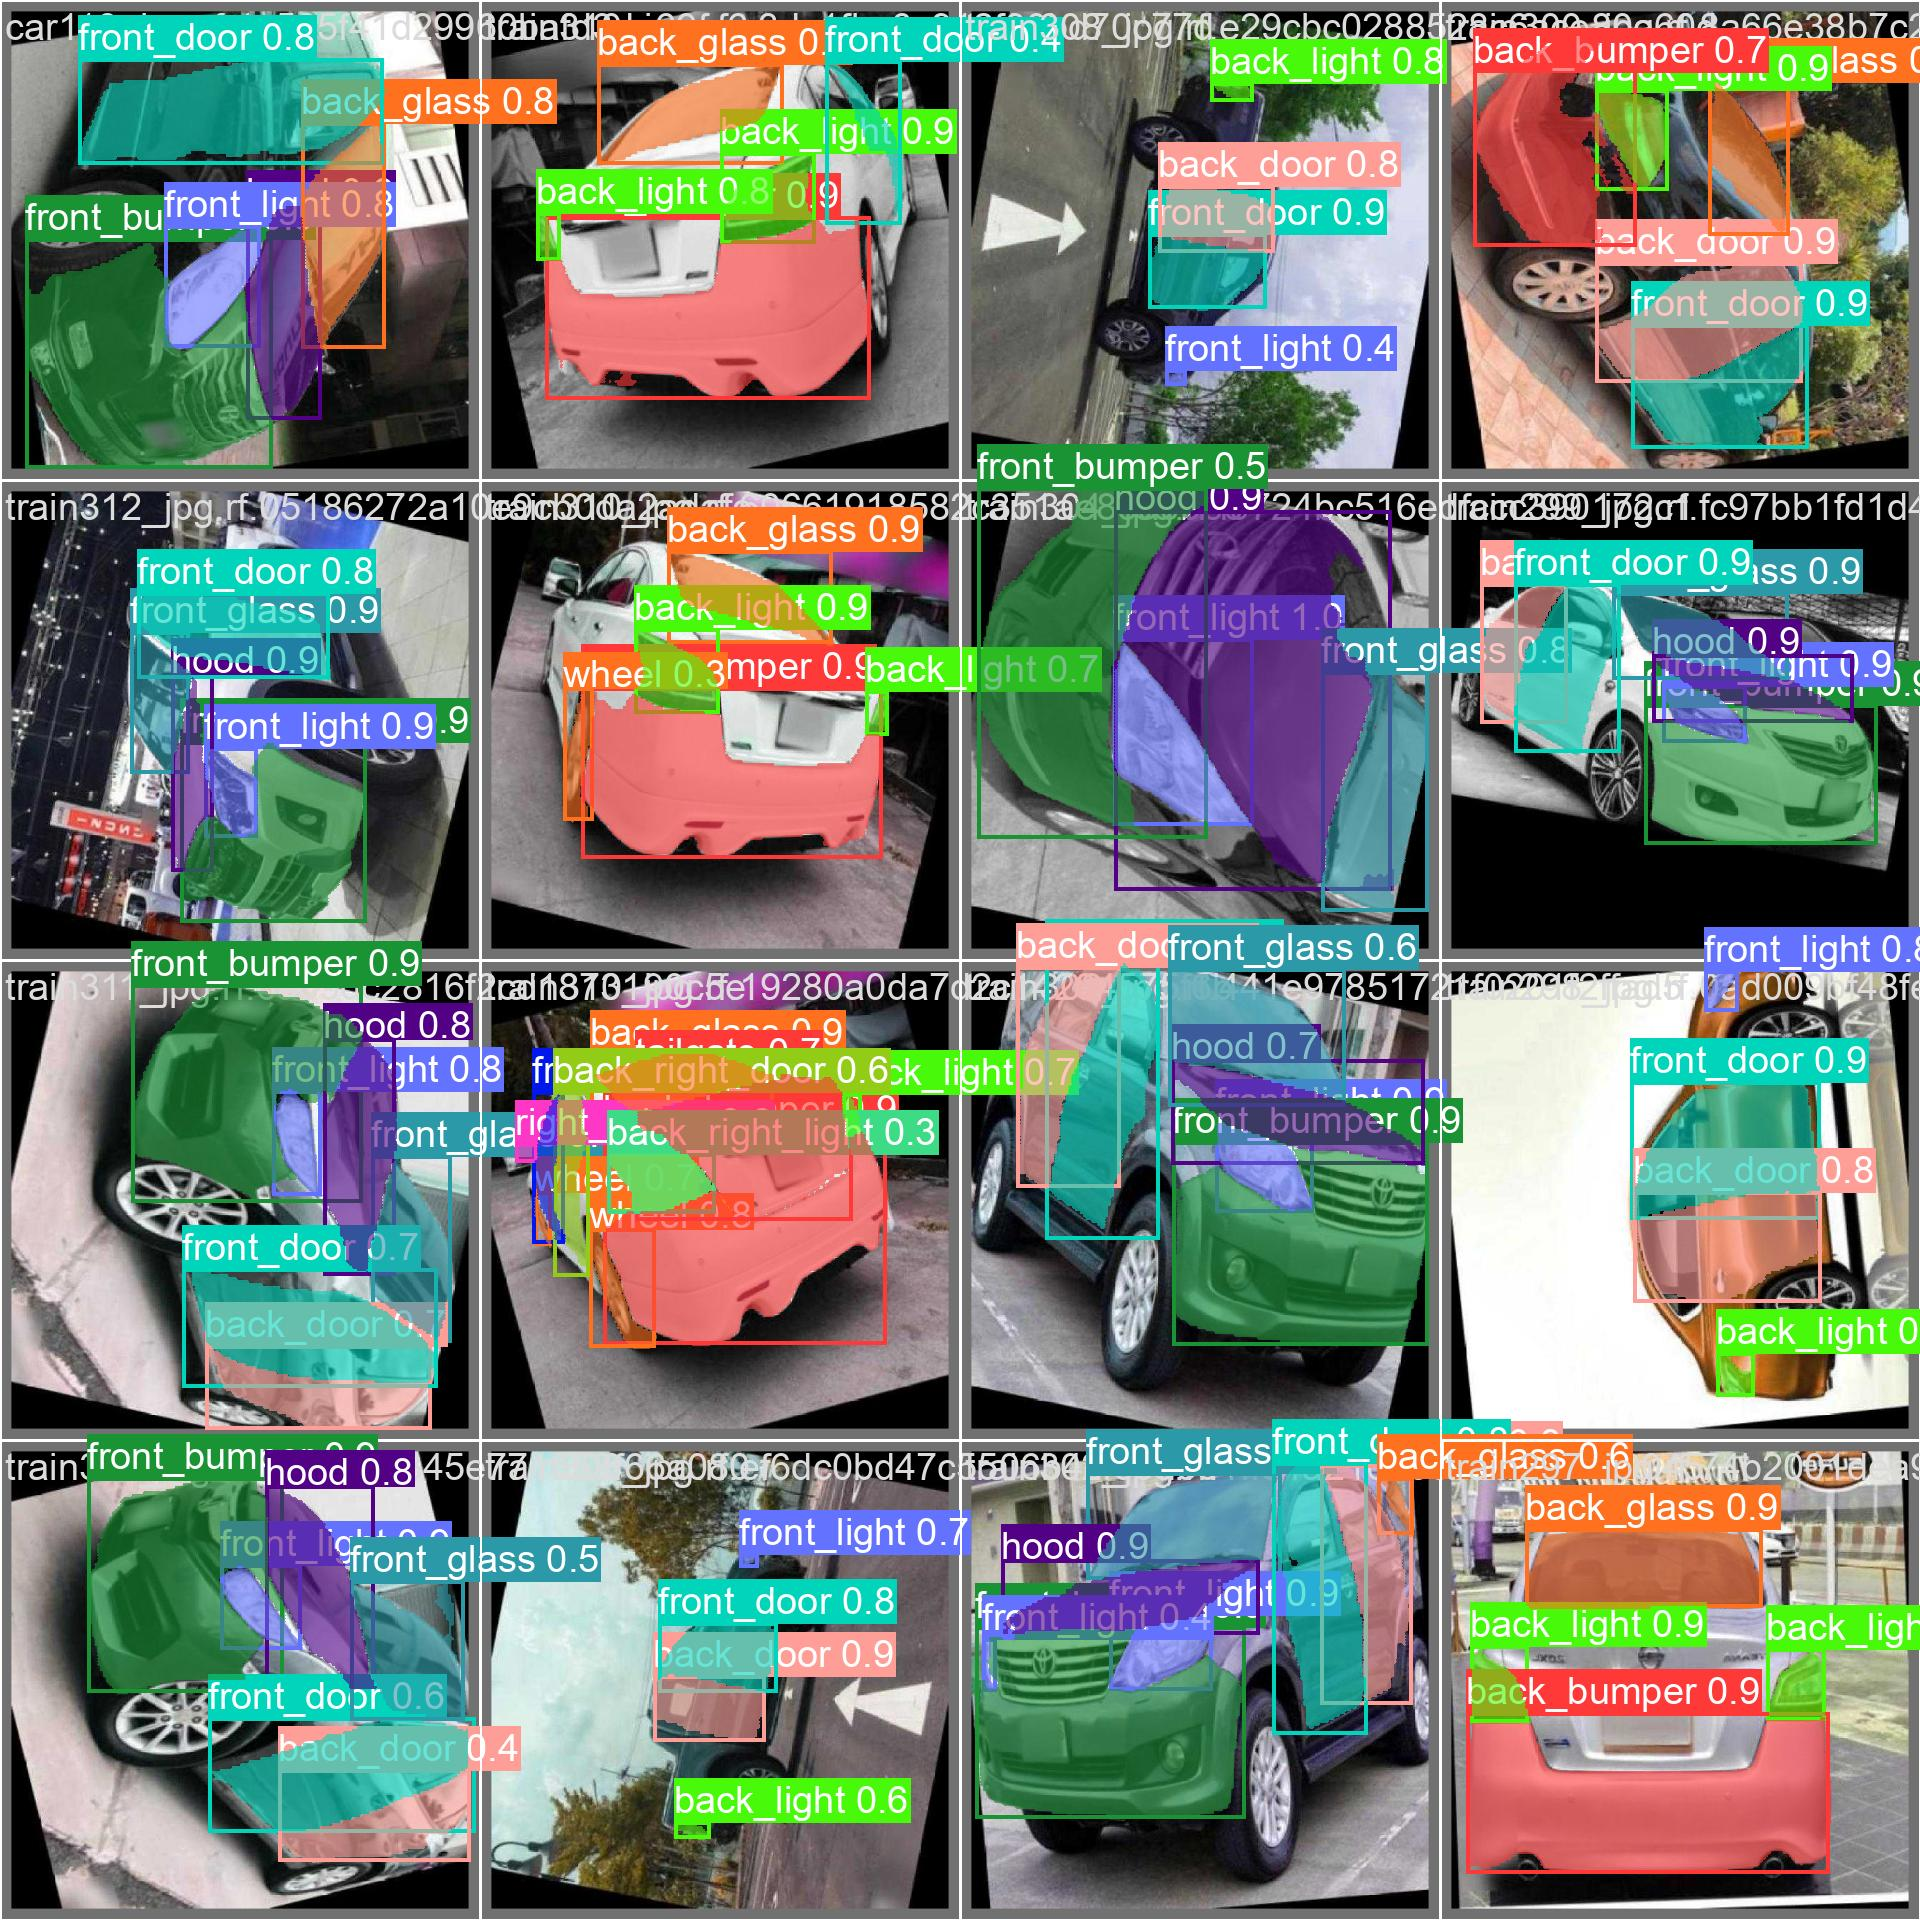
\includegraphics[width=0.7\columnwidth]{images/ema_wiou.jpg}
				\caption{YOLOv8 with EMA and WIoU segmentation}
			\end{figure}
		\end{column}
	\end{columns}
\end{frame}

\subsection{Deep Snake, Flexible Design}
\begin{frame}{Inprovement: Deep Layer Aggregation}
	\begin{figure}[h]
		\centering
		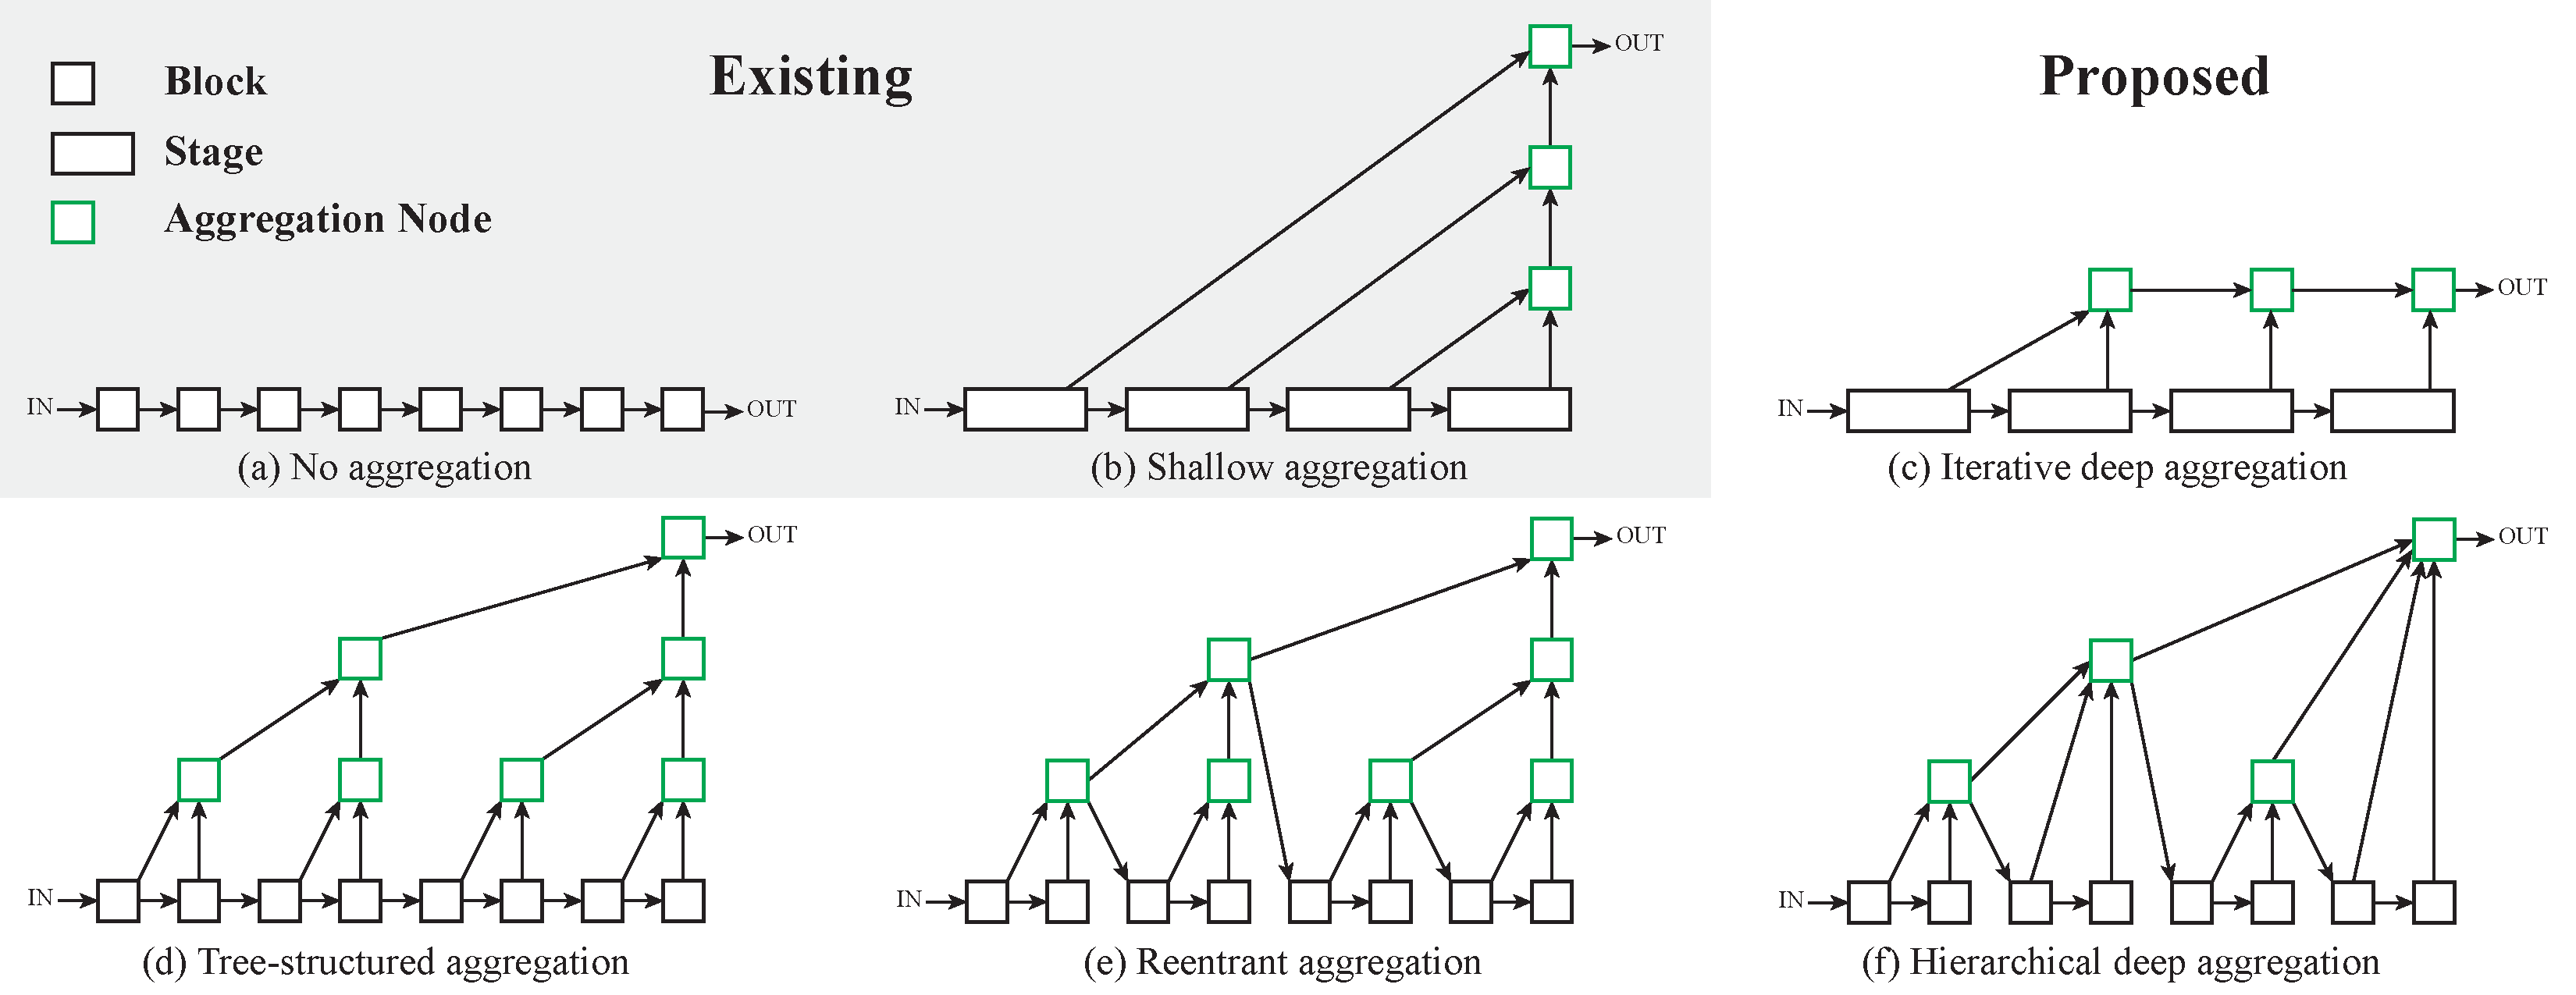
\includegraphics[width=0.9\textwidth]{images/diff_aggregation.pdf}
		\caption{Different ways to aggregate layers}
		\label{fig:diff_aggregation}
	\end{figure}
\end{frame}

\begin{frame}{Inprovement: Deep Layer Aggregation}
	\begin{figure}[h]
		\centering
		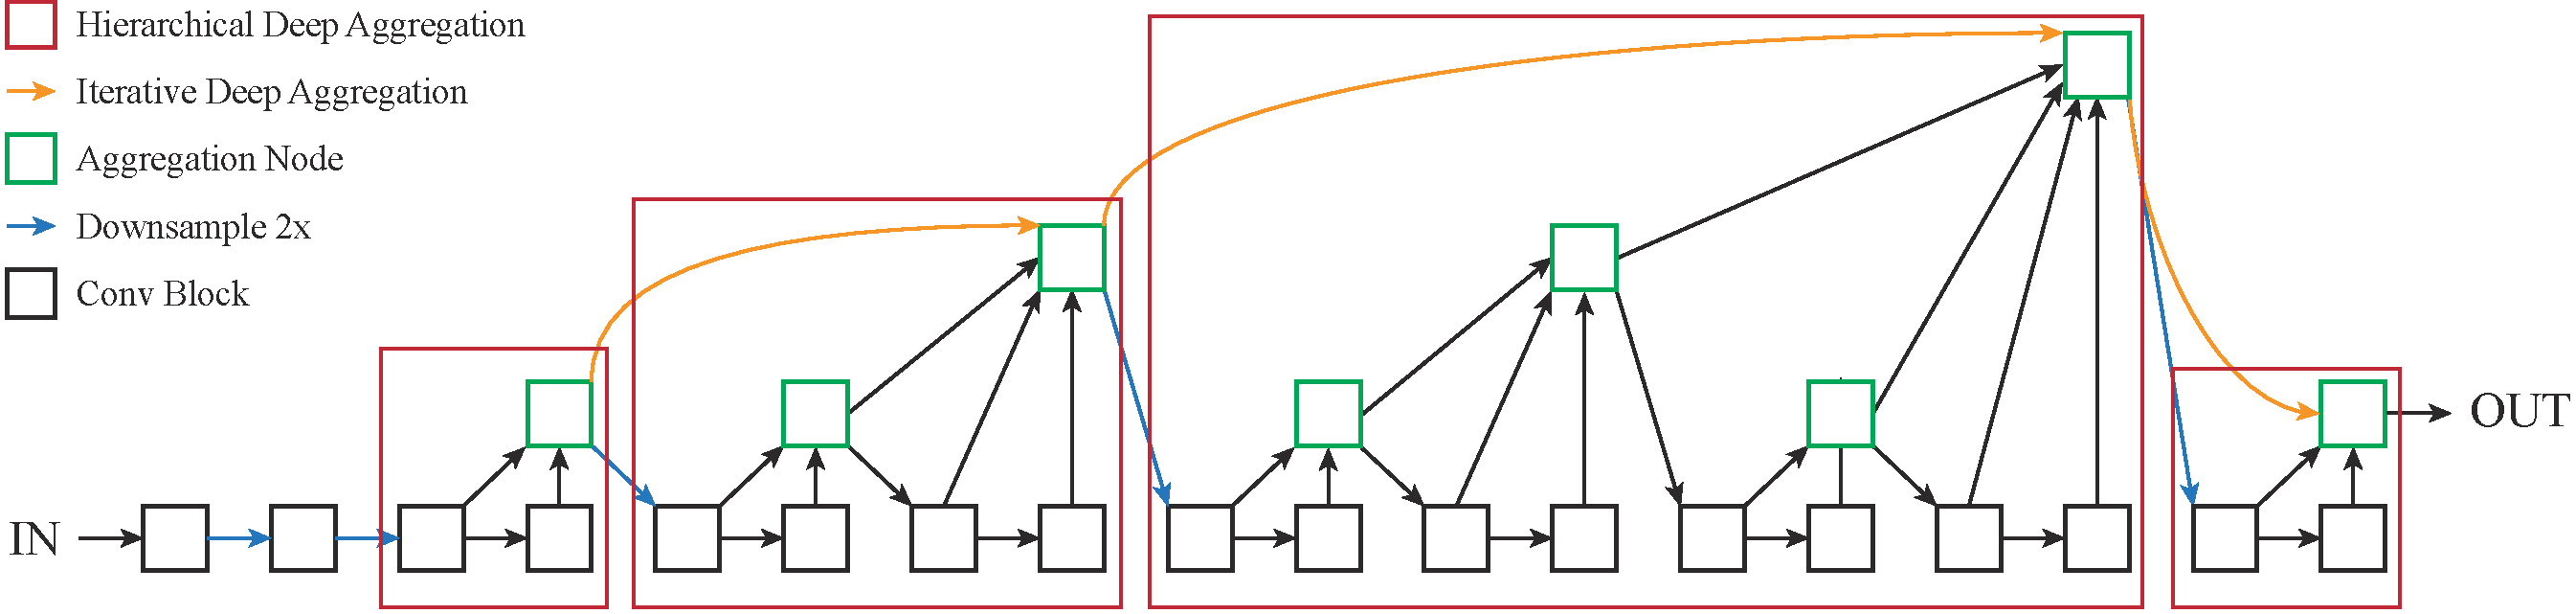
\includegraphics[width=\textwidth]{images/dla_architecture.pdf}
		\caption{DLA network architecture}
		\label{fig:dla_architecture}
	\end{figure}
\end{frame}

\begin{frame}{Experiment: Deep Snake}
	\begin{figure}[h]
		\centering
		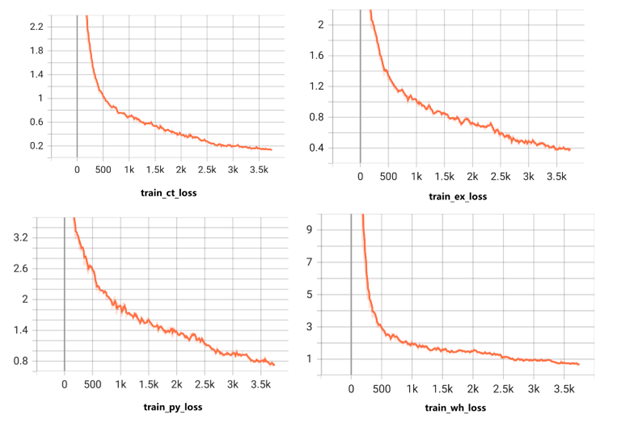
\includegraphics[width=0.7\textwidth]{images/train_loss.png}
		\caption{Loss during training}
		\label{fig:train_loss}
	\end{figure}
\end{frame}

\begin{frame}{Experiment: Deep Snake}
	\begin{figure}[h]
		\centering
		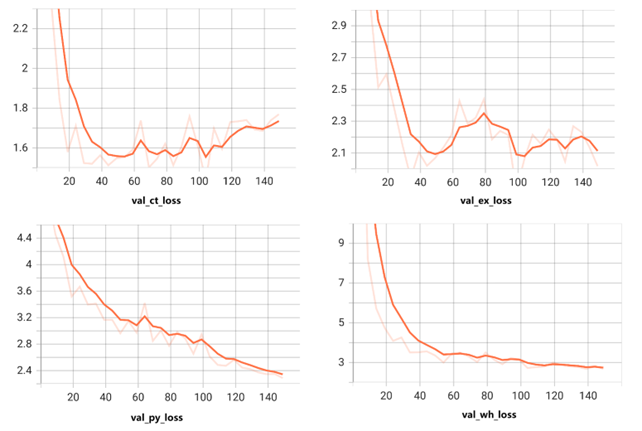
\includegraphics[width=0.7\textwidth]{images/val_loss.png}
		\caption{Loss during validation}
		\label{fig:val_loss}
	\end{figure}
\end{frame}

\begin{frame}{Experiment: Deep Snake}
	\begin{figure}[h]
		\centering
		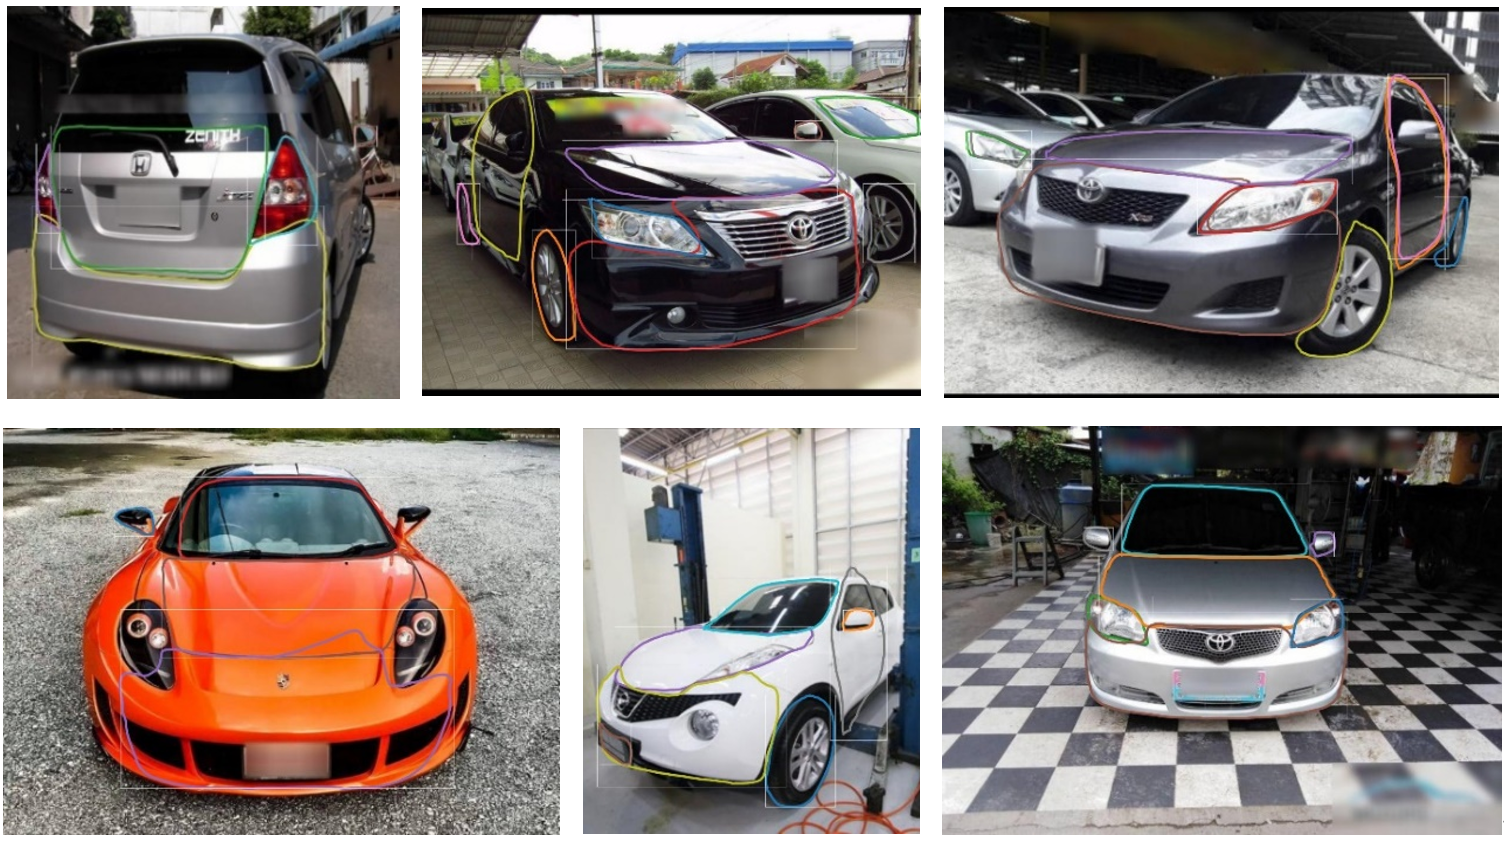
\includegraphics[width=0.8\textwidth]{images/deepsnake_demo.png}
		\caption{Sample pictures segmented by Deep Snake}
		\label{fig:deepsnake_demo}
	\end{figure}
\end{frame}

%\begin{frame}[plain, allowframebreaks, noframenumbering]{Content}
%	\tableofcontents
%\end{frame}
%
%\section{Conclusion}

\begin{frame}{总结展望}
	\begin{block}{你好}
		那就这样吧
	\end{block}
\end{frame}

% 致谢页面
{
    \usebackgroundtemplate{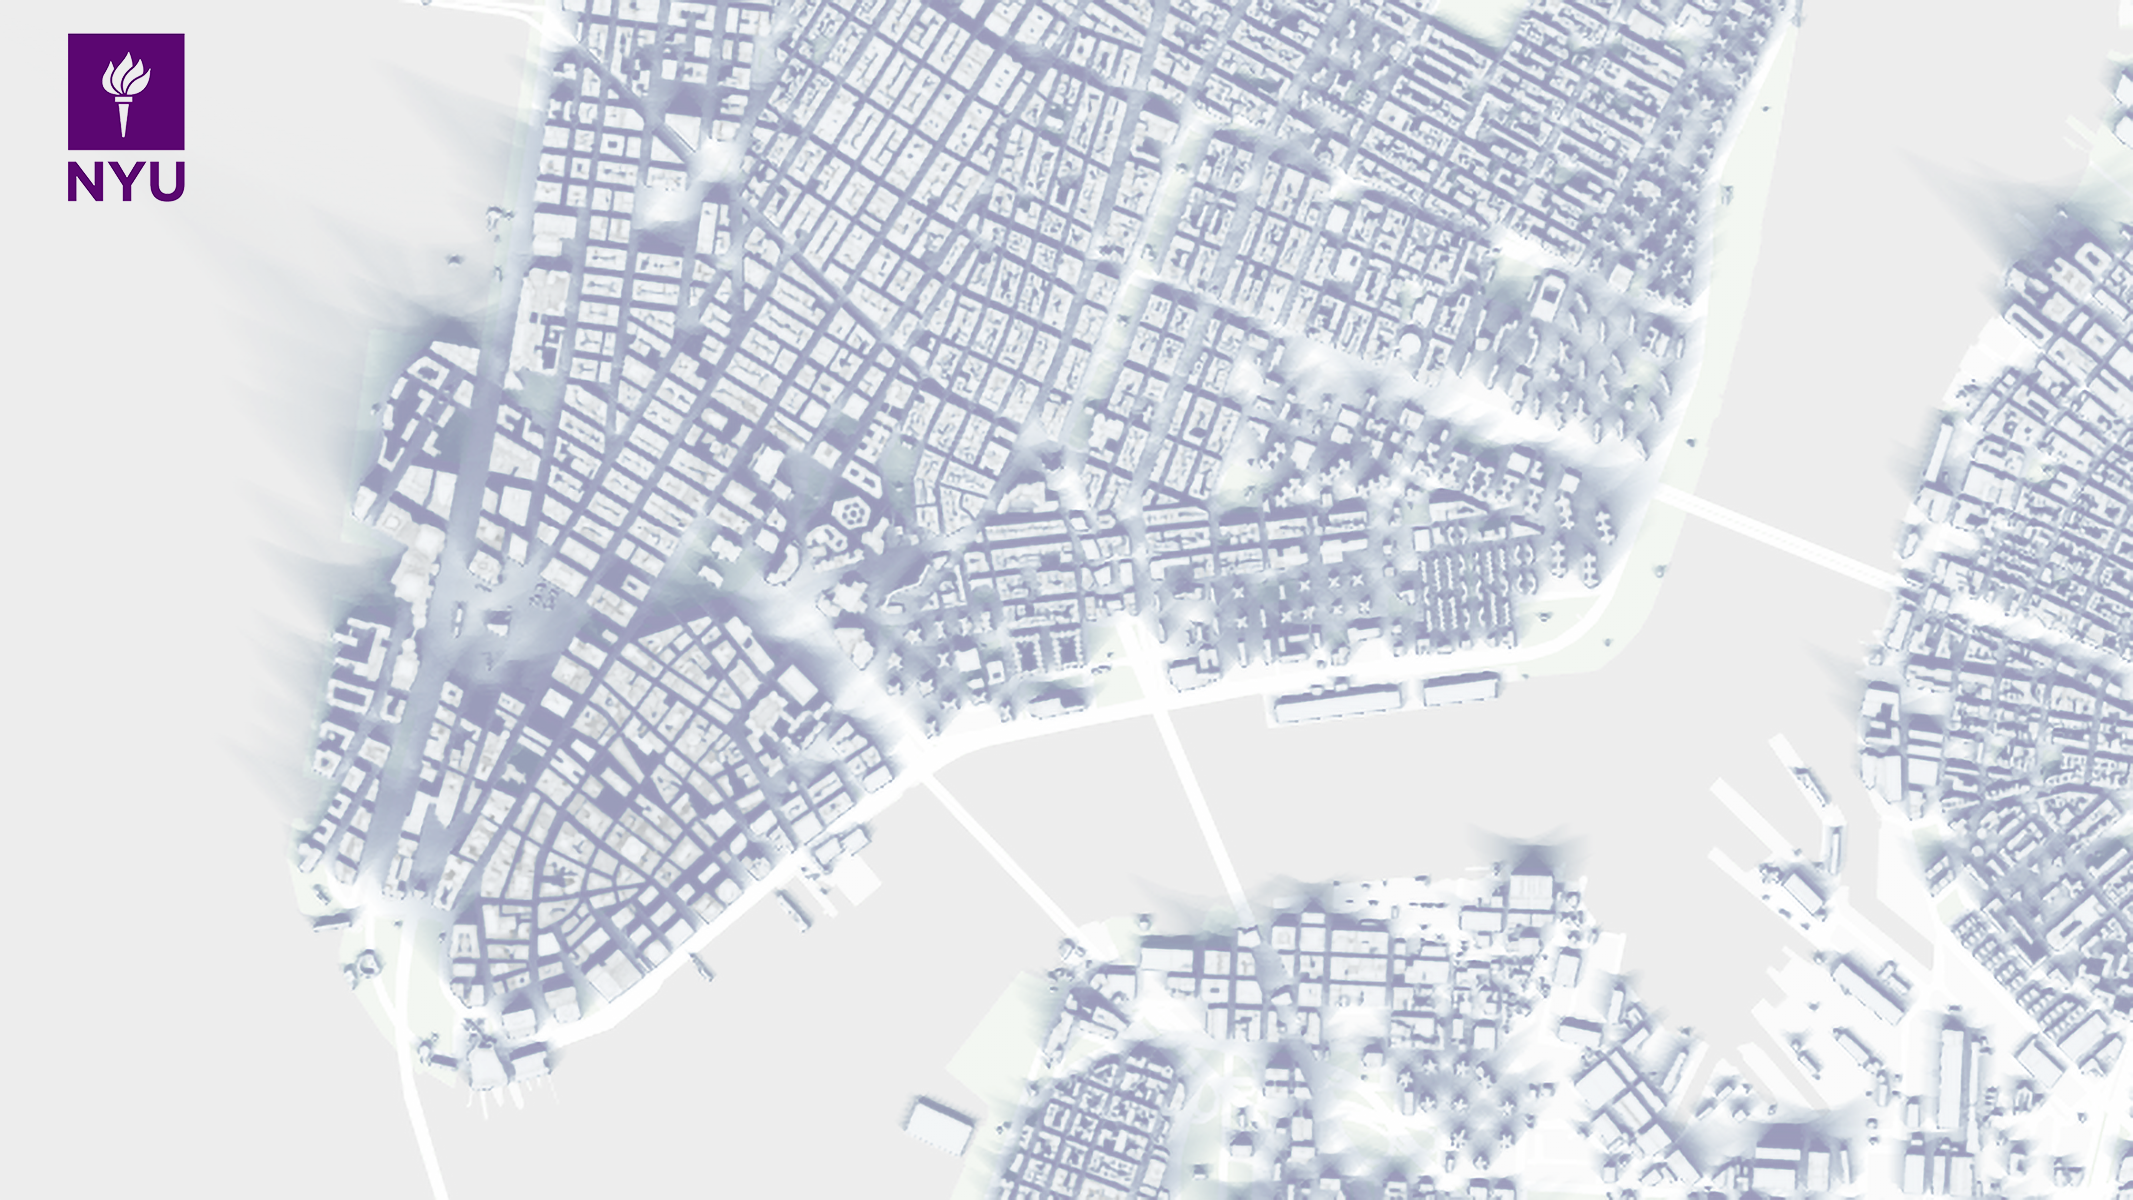
\includegraphics[width=\paperwidth]{background_purple_nyu.png}} % 背景图片
    \usebeamercolor{structure}
    \begin{frame}[plain]
        \begin{center}
            \textcolor{fg}{\Huge \textbf{THANK YOU}}
%            \vskip 1cm
%            \textcolor{fg}{\large 焚膏油以继晷,恒兀兀以穷年。}
        \end{center}
    \end{frame}
}

\end{document}


